% \documentclass{article}
% 
% \usepackage{etoolbox}
% 
% \usepackage{verbatim}
% \usepackage{graphicx}
% \usepackage{amsmath,amsfonts,amssymb,latexsym}
% \usepackage{color}
% \usepackage{flushend}
% \usepackage{subfigure}
% \usepackage{multicol}
% \usepackage{hhline}
% \usepackage{cite}
% \usepackage[table]{xcolor}
% \usepackage{mathptmx}
% \usepackage{hyperref} 
% 
% \usepackage{macros}
% \usepackage[ruled]{algorithm}
% \usepackage{algpseudocode}
% \usepackage{ioa_code}
% 
% \newtheorem{definition}{Definition}
% \newtheorem{theorem}{Theorem}
% \newtheorem{lemma}{Lemma}
% \newtheorem{corollary}{Corollary}
% \newcommand{\toto}{xxx}
% \newenvironment{proofT}{\noindent{\bf
% Proof }} {\hspace*{\fill}$\Box_{Theorem~\ref{\toto}}$\par\vspace{3mm}}
% \newenvironment{proofL}{\noindent{\bf
% Proof }} {\hspace*{\fill}$\Box_{Lemma~\ref{\toto}}$\par\vspace{3mm}}
% \newenvironment{proofC}{\noindent{\bf
% Proof }} {\hspace*{\fill}$\Box_{Corollary~\ref{\toto}}$\par\vspace{3mm}}
% 
% \newenvironment{proof}{\noindent{\bf Proof.}}{\hfill$\Box${\vspace*{\medskipamount}}}
% 
% \newcommand{\remove}[1]{}
% \newcommand{\vincent}[1]{{\bf [V: #1]}}
% \newcommand{\michel}[1]{{\bf [M: #1]}}
% \newcommand{\tyler}[1]{{\bf [T: #1]}}
% \usepackage{umr-V2}
% \RRtitle{Un arbre binaire de recherche d\'edi\'e aux acc\`es transactionnels}
% \RRetitle{A Speculation-Friendly Binary Search Tree\thanks{A 2-column 10 page version appeared at the 17th ACM SIGPLAN
% Symposium on Principles and Practice of Parallel Programming (PPoPP 2012), ACM press.}}
% \RRauthor{
% \vspace{-1em}
% Tyler Crain\thanks{Projet ASAP : \'equipe commune avec l'INRIA, le CNRS, l'universit\'e de Rennes 1},
% Vincent Gramoli\thanks{EPFL}
% Michel Raynal\thanks{Projet ASAP : \'equipe commune avec l'INRIA, le CNRS, l'universit\'e de Rennes 1; Senior member, Institut Universitaire de France}
% \\
% {\it tyler.crain@irisa.fr, vincent.gramoli@epfl.ch, raynal@irisa.fr}
% }
% \authorhead{T. Crain, V. Gramoli \& M. Raynal}
% \titlehead{A Transaction-Friendly Binary Search Tree} 
% \RRnote{        
% }
% \RRdate{septembre 2011}
% \RRNo{1984}
% \RRresume{Les transactions, qui utilisent une technique de synchronisation optimiste,
% simplifient la programmation des architectures multi-c\oe{}urs.
% En effet, un programmeur a seulement besoin d'ins\'erer des op\'erations dans des transactions afin
% d'obtenir un programme concurrent correct. Les programmeurs ont donc tout naturellement utilis\'e
% cette encapsulation sur plusieurs structures de donn\'ees originellement d\'edi\'ees \`a la programmation pessimiste
% (non optimistes) pour \'evaluer les transactions. L'exemple le plus probant \'etant l'arbre transactionnel rouge-noir
% d\'evelopp\'e par Oracle Labs et pr\'esent dans plusieurs distributions.
% 
% Malheureusement, ces structures de donn\'ees ne sont pas adapt\'ees \`a des ex\'ecutions optimistes car elles reposent
% sur des invariants contraignants, comme la profondeur logarithmique d'un arbre, pour borner le co\^ut des
% acc\`es pessimistes. Une telle complexit\'e ne s'applique pas aux acc\'es optimistes et garantir de tels
% invariants n'est pas n\'ecessaire et induit de la contention en augmentant la probabilit\'e pour une transaction 
% d'avorter et de recommencer.
% 
% Dans ce papier, nous pr\'esentons un arbre binaire de recherche qui viole de fa\c{c}on transitoire ces invariants
% pour gagner en efficacit\'e. Nous montrons que cet arbre est plus efficace que les arbres AVL et rouge-noir.
% Sa nouveaut\'e majeure r\'eside dans la s\'eparation de ses op\'erations de modifications : elles sont coup\'ees en une transaction qui modifie
% l'abstraction et plusieurs autres qui restructurent son impl\'ementation. La biblioth\`eque qui en r\'esulte limite la quantit\'e d'avortements
% en augmentant l\'eg\`erement le nombre d'acc\`es, en particulier, elle am\'eliore une application de r\'eservation de voyage bas\'ee sur les
% transactions par un facteur multiplicatif de 3,5.} 
% \RRmotcle{m\'emoire transactionnelle, arbre binaire, structures de donn\'ees concurrente}
% \RRabstract{We introduce the first binary search tree algorithm designed for speculative executions.
% Prior to this work, tree structures were mainly designed for their pessimistic (non-speculative) accesses to have 
% a bounded complexity. 
% Researchers tried to evaluate transactional memory using such tree structures
% whose prominent example is the red-black tree library developed by Oracle Labs that is part of multiple benchmark distributions. Although well-engineered, such structures remain badly suited for speculative accesses, whose step complexity might raise dramatically with contention.
% 
% We show that our \emph{speculation-friendly tree} outperforms the existing 
% transaction-based version of the AVL and the red-black trees. 
% Its key novelty stems from the \emph{decoupling} of update operations: they are split 
% into one transaction that modifies the abstraction state and multiple ones that restructure its tree 
% implementation in the background.
% In particular, the speculation-friendly tree is shown correct, reusable and
% it speeds up a 
% transaction-based travel reservation application by up to $3.5\times$.}
% \RRkeyword{Transactional Memory, concurrent data structures, balanced binary trees}
% 
% \begin{document}
% \makeRR					

\section{Introduction}

As briefly mentioned in the introduction a partial solution to the difficulty of concurrent programming
is to provide concurrent libraries of popular abstractions.
Generally these are finely tuned high performance libraries
providing the programmer with useful operations.
The implementations of such libraries are often very complex
and difficult to understand, but are provided with a simple to use
interface for anyone to use.
By doing this experts can create algorithms providing strong guarantees
and good performance that can then be widely reused.

In an optimal situation transactional memory would not need such libraries,
as one could just directly place a sequential implementation of an abstraction
directly in transactions and it would perform as well and provide the same
guarantees as a library provided by an expert.
Unfortunately this is not completely true.
Due to the general nature
of the synchronization required by STM, a sequential data structure implementation directly
placed in transactions will never perform as well as a highly tuned concurrent
(lock based or non-blocking) implementation of a data structure done by an expert.
The reason for this is that an expert can consider the specific synchronization needed to implement
that specific data structure safely.

Fortunately this does not mean that data structures in STM will always have suboptimal performance,
instead this gives us the opportunity to design libraries designed specifically for use inside
of transactions that take into account the synchronization considerations
of STM.
By doing this we can provide a programmer using transactions with abstractions that perform closer
to highly optimized non-transactional ones.

A further advantage of providing efficient libraries in STM is given by the reusable nature of code implemented using
transactions, a programmer can use the operations of the abstractions along with his own code
to create new efficient atomic operations.
For example a programmer might use a map abstraction that provides an $\lit{insert}$ and a $\lit{delete}$ operation
to create an atomic $\lit{move}$ operation by simply combing the $\lit{insert}$ and $\lit{delete}$ in a transaction.

By providing a programmer with a large selection of transaction based implementations of commonly used abstractions
his life becomes much easier.
Accordingly, this chapter will focus on designing efficient data structures in transactional memory (specifically those providing the map abstraction).
Even though the previous chapters focused on considering how to define transaction semantics so that the programmer can use them easily and
the data structures presented in this chapter are not directly related to programmers interaction with transaction semantics,
this chapter still focuses on dealing with the ease of use of the STM ecosystem.
Namely, it promotes the fact that the proposed data structures can help increase the ease of use of STM for concurrent programming.
As sated in the discussion of the STM abstraction in the introduction (specifically Definition \ref{def:stm-def}), the desired STM abstraction
should exist as a one component of the concurrent system as a whole, therefore providing libraries implementing additional abstractions
that are able to execute within the STM helps constitute this easy to use ecosystem; similar to the way the \emph{java.util.concurrent}
package as part of the Oracle Java SDK \cite{javasdk} provides several different lock type abstractions in addition to many concurrent data structure
implementations.
Furthermore, if these STM compatible libraries provide good performance they give an additional reason to use STM as an attractive alternative to
concurrent code using locks or even highly tuned non-blocking abstractions.
The reason for this is that the programmer can reuse
the STM compatible libraries directly within his transactions in order to compose new atomic operations specific to his needs,
something that is usually not possible using lock based or non-blocking abstractions.


% % multicore data structure
% The multicore era is changing the way we write concurrent programs.
\paragraph{Concurrent data structures}
In this multicore era, concurrent data structures are becoming important building blocks
for programmers writing concurrent programs.
They present the programmer with a clear interface to a given abstraction, allowing
him to safely perform operations to the abstraction in a concurrent context.
Due to their importance in organizing data between processes they are increasingly becoming a bottleneck
in a wide variety of concurrent applications.
Considering data structures in general, both concurrent and sequential, they often rely on keeping invariants
in order to ensure their efficiency and big-O complexity.
In the case of a tree, it must typically remain sufficiently balanced at any point of the concurrent execution.
Unfortunately while these invariants are important to keep, they can also prevent
the performance from scaling with multiple cores~\cite{Sha2011}.

% New programming constructs like transactions~\cite{HM93,ST97} promise 
% to exploit the concurrency inherent to multicore architectures.
% Most transactions build upon \emph{optimistic synchronization}, 
% where a sequence of shared accesses is executed speculatively and might abort.
% They simplify concurrent programming for two reasons.
% First, the programmer only needs to delimit regions of sequential 
% code into transactions or to replace critical sections by transactions
% to obtain a safe concurrent program.
% Second, the resulting transactional program is reusable by any programmer, 
% hence a programmer composing operations from a transactional library into another 
% transaction is guaranteed to obtain new deadlock-free operations that execute atomically.
% By contrast, \emph{pessimistic synchronization}, where each access to some 
% location $x$ blocks further accesses to $x$,
% is harder to program with~\cite{PA11,RHW10} and hampers reusability~\cite{HMPH05,GG11}.

% problem
Further aggrandizing this problem, it is unclear how one can adapt a data structure to 
access it efficiently through transactions in an STM system.
Potentially as a drawback of the simplicity of using transactions, 
data structures used in transactional memory are most commonly just
their sequential versions pasted directly into transactions.
% as a drawback of the simplicity of using transactions, 
As a consequence of this, existing transactional programs spanning from low level libraries of data structures to 
topmost applications directly derive from sequential or pessimistically synchronized programs.
In this case, not only are the impacts of optimistic synchronization on sequentially defined data structures
ignored, but their effect on performance is compounded from the bottom level of execution all the way to the top.

\begin{figure}[t]
	\begin{center}
	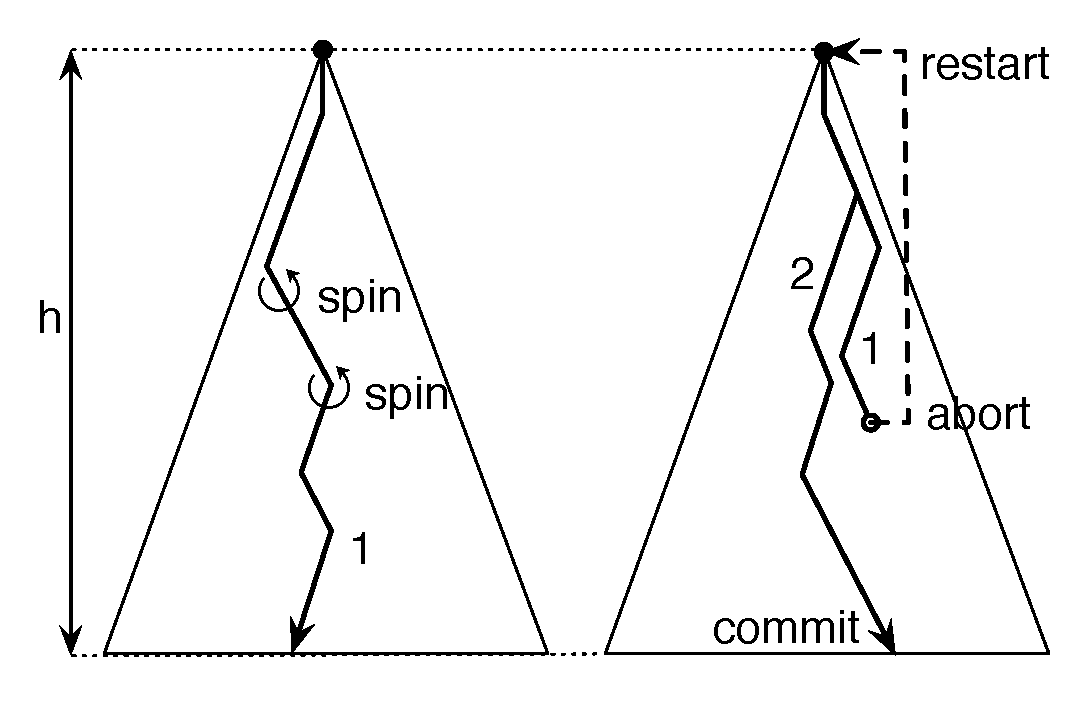
\includegraphics[scale=0.4]{Tree/fig/complexity}
	\caption{A balanced search tree whose complexity, in terms of the amount of accessed elements, is {\bf (left)} proportional to $h$ 
	in a pessimistic execution and {\bf (right)} proportional to the number of restarts in an optimistic execution\label{fig:complexity}}
	\end{center}
\end{figure}

To illustrate the difference between optimistic and pessimistic 
synchronizations consider the example of 
% example
Figure~\ref{fig:complexity} depicting their step complexity when
traversing a tree of height $h$ from its root to a leaf node. On the left, 
steps are executed pessimistically, potentially spinning before being able to acquire 
a lock, on the path converging towards the leaf node. On the right, 
steps are executed optimistically and some of them
may abort and restart, depending on concurrent thread steps. The pessimistic 
execution of each thread is guaranteed to execute $O(h)$ steps, yet the optimistic one 
may need to execute $\Omega(hr)$ steps, where $r$ is the number of restarts. 
Note that $r$ depends 
on the probability of conflicts with concurrent transactions that depends, in turn, 
on the transaction length and $h$.


When implementing a tree using TM it is clear that, although a transaction must be aborted before violating 
the abstraction implemented by this tree
(e.g., inserting $k$ successfully in a set where $k$ has already been inserted by a concurrent transaction),
it is unclear whether a transaction must be aborted due to
slightly unbalancing the tree implementation in order to strictly preserve the balance invariant.
Following this assumption we introduce a \emph{speculation-friendly} tree as a tree that transiently breaks its
balance structural invariant without hampering the abstraction consistency in order to speed up transaction-based accesses. 
% Here are our contributions.
% 
% \begin{itemize}
% \item We propose a speculation-friendly binary search tree data structure
% implementing an associative array and set abstractions.
% In this implementation we decoupling the operations that modify the abstraction (we call these \emph{abstract transactions}) from operations
% that modify the tree structure itself but not the abstraction (we call these \emph{structural transactions}).
% An abstract transaction either inserts or deletes an element from the abstraction and 
% in certain cases the insertion might also modify the tree structure.
% Structural transactions have two main tasks:
% (1) Certain structural transactions are given the task to rebalance the tree 
% by executing a distributed rotation mechanism: each of these transactions executes a local rotation involving
% only a constant number of neighboring nodes. 
% (2) Some other structural transactions unlink and free nodes that have been logically deleted 
% by previously committed abstract transactions.
% 
% \item We prove the correctness (i.e., linearizability) of our tree and we compare its performance against existing transaction-based versions of an AVL tree and a red-black tree,
% widely used to evaluate transactions~\cite{DSS06,HLMS03,CCKO08,HK08,FFR08,YNW+08,DFGG11}.
% The speculation-friendly tree improves by up to $1.6\times$ the performance of the AVL tree on the micro-benchmark and 
% by up to $3.5\times$ the performance of the built-in red-black tree on a travel reservation application, already well-engineered for transactions.
% Finally, our speculation-friendly tree performs similarly to a non-rotating tree but remains robust in face of non-uniform workloads.
% 
% \item We illustrate (i)~the portability of our speculation-friendly tree by evaluating it on two different Transactional Memories (TMs), TinySTM~\cite{FFR08} 
% and $\mathcal{E}$-STM~\cite{FGG09} and with different configuration settings, hence outlining that our performance benefit is independent 
% from the transactional algorithm it uses; and (ii)~its reusability by composing 
% straightforwardly the $\lit{remove}$ and $\lit{insert}$ into a new $\lit{move}$ operation.
% In addition, we compare the benefit of relaxing data structures into speculation-friendly ones against the benefit of only relaxing transactions,
% by evaluating elastic transactions.
% It shows that, for a particular data structure, refactoring its algorithm is preferable to refactoring the underlying transaction algorithm.
% \end{itemize}
% 
% The chapter is organized as follows. In Section~\ref{sec:pb} we describe the problem related
% to the use of transactions in existing balanced trees. In Section~\ref{sec:tf} we present our 
% speculation-friendly binary search tree. In Section~\ref{sec:expe} we evaluate our tree
% experimentally and illustrate its portability and reusability.
% In Section~\ref{sec:rw} we describe the related work and 
% Section~\ref{sec:conclusion} concludes.

\section{The Problem with Balanced Trees}\label{sec:pb}

In this section, we focus our attention 
on the structural invariant of existing tree libraries, namely 
the \emph{balance}, examining the impact of restructuring, namely the \emph{rebalancing}, on contention.

Trees provide logarithmic access time complexity given that they are balanced, 
meaning that among all downward paths from the root to a leaf, the length of the shortest path 
is not far apart the length of the longest path. Upon tree update, if their difference exceeds a given threshold, the structural invariant is broken and a rebalancing is triggered to restructure accordingly. 
%
This threshold depends on the considered algorithm: AVL trees~\cite{AVL62} do not tolerate 
the longest length to exceed the shortest by 2 whereas red-black trees~\cite{Bay72} tolerate 
the longest to be twice the shortest, thus restructuring less frequently.  Yet in both cases
the restructuring is triggered immediately when the threshold is reached to hide the imbalance from further operations.

Generally, one takes an existing tree algorithm and encapsulates all its accesses within transactions 
to obtain a concurrent 
tree whose accesses are guaranteed atomic (i.e., linearizable), however, 
the obtained concurrent transactions likely \emph{conflict} (i.e., one accesses the same 
location another is modifying), resulting in the need to abort one of these transactions which leads to  a significant waste of efforts.
This is in part due to the fact that encapsulating an \emph{update} operation (i.e., an $\act{insert}$ or a $\act{remove}$ operation)
into a transaction boils down to encapsulating four phases in the same transaction:
\begin{enumerate}
	\item the modification of the abstraction, 
	\item the corresponding structural adaptation,
	\item a check to detect whether the threshold is reached and 
	\item the potential rebalancing.
\end{enumerate}

\paragraph{A transaction-based red-black tree}
An example is the transaction-based binary search tree developed by Oracle Labs (formerly Sun Microsystems) and other researchers 
to extensively evaluate transactional memories~\cite{DSS06,HLMS03,CCKO08,HK08,FFR08,YNW+08,DFGG11} .
This library relies on the classical red-black tree algorithm that bounds the step complexity of pessimistic $\act{insert}$/$\act{delete}$/$\act{contains}$.
It has been slightly optimized for transactions by removing sentinel nodes to reduce false-conflicts, and we are aware of 
two benchmark-suite distributions that integrate it, STAMP~\cite{CCKO08} and synchrobench\footnote{http://lpd.epfl.ch/gramoli/php/synchrobench.php}.


\begin{figure*}
	\begin{center}
	\subfigure[Initial tree\label{sfig:tree1}]{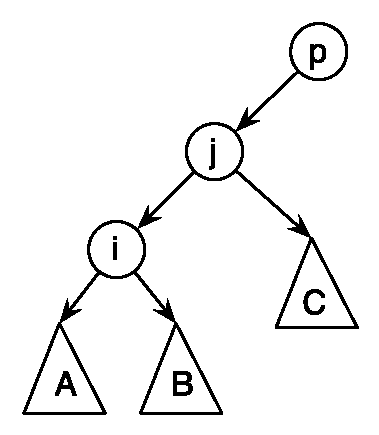
\includegraphics[scale=0.6]{Tree/fig/tree1b}}\hspace{4em}
	\subfigure[Result of a classical right rotation\label{sfig:tree2}]{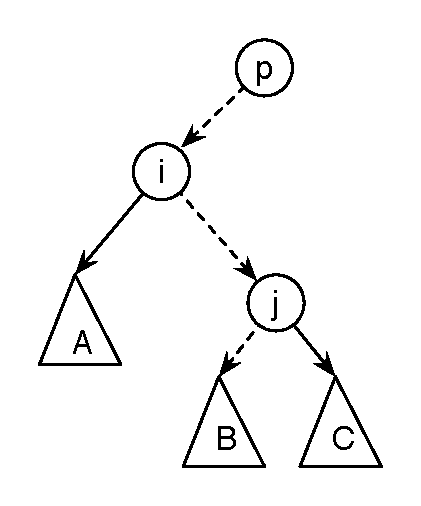
\includegraphics[scale=0.6]{Tree/fig/tree2b}}\hspace{4em}
	\subfigure[Result of the new right rotation\label{sfig:tree3}]{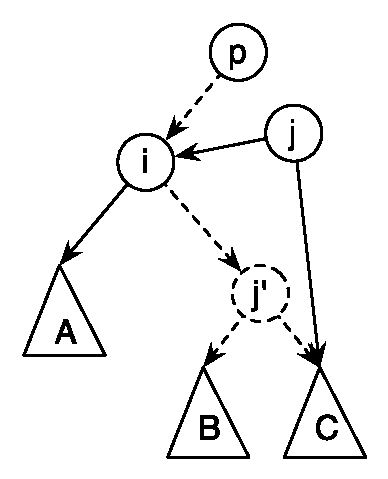
\includegraphics[scale=0.6]{Tree/fig/tree3b}}
	\caption{The classical rotation modifies node $j$ in the tree and forces a concurrent traversal at this node to backtrack; the new rotation left $j$ unmodified, adds $j'$ and postpones the 
	physical deletion of $j$\label{fig:rotation}}
	\end{center}
\end{figure*}


Each of its update transactions encapsulate all the four phases given above even though phase (1) could be decoupled 
from phases (3) and (4) if transient violations of the balance invariant were tolerated.
Such a decoupling is appealing given that phase (4) is subject to conflicts.
In fact, the algorithm balances the tree by executing rotations starting from the position where a node is inserted or deleted 
and possibly going all the way up to the root. As depicted in Figure~\ref{fig:rotation}(a) and (b), a rotation consists of 
replacing the node where the rotation occurs by the child and adding this replaced node to one of its subtrees.
A node cannot be accessed concurrently by an abstract transaction and a rotation, otherwise the abstract transaction might miss the node it 
targets while being rotated downward. Similarly, rotations cannot access common nodes as one rotation may unbalance the others.

Moreover, the red-black tree does not allow any abstract transaction to access a node that is concurrently being deleted from the abstraction because
phases (1) and (2) are tightly coupled within the same transaction.
If this was allowed the abstract transaction's traversal might end up on the node that is no longer part of the tree.
Fortunately, if the modification operation is a deletion, then phase (1) can be decoupled from the structural modification of phase (2)
by marking the targeted node as logically deleted in phase (1) effectively removing it from the set abstraction prior to unlinking it physically in phase (2).
This improvement is important as it lets a concurrent abstract transaction can travel through the node concurrently being logically deleted in phase (1) without conflicting.
%\tyler{Then remove this: This improvement is important to let a $\act{contains}$ access a node that is concurrently being logically deleted in phase (1).}
Making things worse, without decoupling these four phases, having to abort within phase (4) would typically require the three previous phases 
to restart as well. 
Finally without decoupling only $\act{contains}$ operations are guaranteed not to conflict with each other.
With decoupling, $\act{insert}$/$\act{delete}$/$\act{contains}$ do not conflict with each other unless they terminate on the same node as described in Section~\ref{sec:tf}.

To conclude, for the transactions to preserve the atomicity and invariants of such a tree algorithm, they typically have to 
keep track of a large \emph{read set} and \emph{write set}, 
i.e., the sets of accessed memory locations that are protected by a transaction. 
Possessing large read/write sets increases the probability of conflicts and thus reduces concurrency.
This is especially problematic
in trees because the distribution of nodes in the read/write set is skewed so that the
probability of the node being in the set is much higher for nodes near the root and the root is guaranteed to be in the read set,
resulting in any transaction that modifies the structure at the root creating conflicts with all live transactions.

\paragraph{Illustration}

To briefly illustrate the effect of tightly coupling update operations on the step complexity of classical transactional balanced trees
we have counted the maximal number of reads necessary to complete typical $\lit{insert}$/$\lit{remove}$/$\lit{contains}$ operations.
Note that this number includes the reads executed by the transaction each time it aborts in addition to the read set size of the transaction obtained at commit time.

%\renewcommand{\tabcolsep}{3.45pt}
\begin{table}[!ht]
 \centering
	\begin{tabular}{|c|c|c|c|c|c|c|}
  \hline
  Update & 0\% & 10\% & 20\% & 30\% & 40\% & 50\%\\  \hline\hline
  AVL tree & 29 & 415 & 711 & 1008 & 1981 & 2081  \\ \hline
  Oracle red-black tree & 31 & 573 & 965 & 1108 & 1484 & 1545   \\ \hline
  Speculation-friendly tree & 29 & 75 & 123  & 120 & 144 & 180   \\ \hline
 \end{tabular}
 \caption{Maximum number of transactional reads per operation on three $2^{12}$-sized balanced search trees as the update ratio increases}
 \label{table:complexity}
\end{table}

We evaluated the aforementioned red-black tree, an AVL tree, 
and our speculation-friendly tree on a 48-core machine using the same transactional memory (TM) algorithm\footnote{TinySTM-CTL, i.e., with lazy 
acquirement~\cite{FFR08}.}.
The expectation of the tree sizes is fixed to $2^{12}$ during the experiments by performing an 
$\lit{insert}$ and a $\lit{remove}$ with the same probability.
Table~\ref{table:complexity} depicts the maximum number of transactional reads
per operation observed among 48 concurrent threads as we increase the update ratio, i.e., the proportion of $\lit{insert}$/$\lit{remove}$ operations over $\lit{contains}$ operations.

For all three trees, the transactional read complexity of an operation increases with the update ratio due to the additional aborted efforts induced by the 
contention. 
Although the red-black and the AVL trees objective is to keep the complexity of pessimistic accesses $O(\log_2 n)$ (proportional to 12 in this case), where $n$ is the tree size,
the read complexity of optimistic accesses grows significantly ($14\times$ more at $10\%$ update than at 0\%, where there are no aborts) as the contention increases.
As described in the sequel, the speculation-friendly tree succeeds in limiting the step complexity raise ($2.6\times$ more at $10\%$ update) of data structure accesses when 
compared against the transactional versions of state-of-the-art tree algorithms.
% An optimization further reducing the number of transactional reads between 2 (for 10\% updates) and 
% 18 (for 50\% updates) is presented in Section~\ref{sec:improvements}.

%\input Tree/alg/simpletree-with-labels.tex


\input Tree/alg/simpletree-with-labels2.tex



\section{The Speculation-Friendly Binary Search Tree}\label{sec:tf}

We introduce the speculation-friendly binary search tree by describing its implementation of an associative array abstraction, mapping a key to 
a value. In short, the tree speeds up the access transactions by decoupling two conflict-prone operations: the node deletion and the tree rotation. 
Although these two techniques have been used for decades in the context of data management~\cite{DLM78,Moh90}, our algorithm novelty lies in applying 
their combination to reduce transaction aborts. We first depict, in Algorithm~\ref{fig:tree-abstract},\ref{fig:tree-maintenance}, the pseudocode that looks like sequential code encapsulated 
within transactions before presenting, in Algorithm~\ref{fig:tree-opt-find}, \ref{fig:tree-opt-maintenance}, more complex optimizations.

\subsection{Decoupling the tree rotation}
The motivation for rotation decoupling stems from two separate observations on traditional tree implementations: (i)~a rotation is tied to the abstract modification
(either successfully adding or removing a node) that triggers it, hence, after the abstract modification the same process
is also responsible for ensuring that its modification does not break the balance invariant and (ii)~a rotation affects different 
parts of the tree apart from where the abstract modification (the location of the node added or removed) took place, hence an isolated conflict can abort the rotation performed at multiple nodes.
In response to these two issues we introduce a dedicated \emph{rotator} thread responsible for eventually ensuring the balance invariant,
allowing transactions performing abstract modifications to complete faster faster and we also distribute the multiple rotations needed to ensure balance 
into single rotation (node-)local transactions. 
Note that our rotating thread is similar to the collector 
thread proposed by Dijkstra et al.~\cite{DLM78} to garbage collect stale nodes.

This decoupling allows the read set of the $\act{insert}$/$\lit{delete}$ operations to only contain the path from the root to the node(s) being modified and the write set to only contain
the nodes that need to be modified in order to ensure the abstraction modification (i.e., the nodes at the bottom of the search path), thus reducing conflicts significantly.
Let us consider a specific example.
If rotations are performed within the $\act{insert}$/$\act{delete}$ operations, then each rotation increases the read and write set sizes.
Take an $\act{insert}$ operation that triggers a right rotation such as the one depicted in Figures~\ref{sfig:tree1}-\ref{sfig:tree2}.
Before the rotation the read set for the nodes $\ms{p},\ms{j},\ms{i}$ is $\{\ms{p.\ell}, \ms{j.r}\}$, where $\ell$ and $r$ represent the left and right pointers, and the write set is $\emptyset$.
Now with the rotation the read set becomes $\{\ms{p.\ell}, \ms{i.r}, \ms{j.\ell}, \ms{j.r}\}$ and the write set becomes $\{\ms{p.\ell}, \ms{i.r}, \ms{j.\ell}\}$
as denoted in the figure by dashed arrows.
Due to $\ms{p.\ell}$ being modified, any concurrent transaction that traverses any part of this section of the tree (including all nodes $i$, $j$, and subtrees $A$, $B$, $C$, $D$)
will have a read/write conflict with this transaction.
In the worst case an $\act{insert}$/$\act{delete}$ operation triggers rotations all the way up to the root resulting in conflicts with all concurrent transactions.

\paragraph{Rotation}

\begin{figure}[h!]
\centering{ \fbox{
\begin{minipage}[t]{150mm}
\footnotesize 
\renewcommand{\baselinestretch}{2.5} 
\resetline
\begin{tabbing}
aaaaa\=aa\=aaaaa\=aa\=aa\=aa\=aa\=\kill %~\\


\bf{operation} $\act{recursive\_balance}(parent, n, left-child)_p$ \\
		\line{MB01} \> \bf{if} ($\ms{n} = \bot$) \bf{then} $\act{return}(0)$ \bf{end if}; \\
		\line{MB01} \> $\ms{\ell} \gets \ms{n.\ell}$; $\ms{r} \gets \ms{n.r}$; \\
		\line{MB01} \> $\ms{n.left-h} \gets \act{recursive\_balance}(\ms{n}, \ms{\ell}, \lit{true})$; \\
		\line{MB01} \> $\ms{n.right-h} \gets \act{recursive\_balance}(\ms{n}, \ms{r}, \lit{false})$; \\
		\line{MB01} \> $\ms{n.local-h} \gets \act{max}(\ms{n.left-h},\ms{n.right-h}) + 1$; \\
		\line{MB01} \> \bf{if} ($\ms{n.left-h} > \ms{n.right-h} + 1$) {\bf then} \\
% 		\line{MB01} \>\> $\ms{\ell} \gets \ms{n.\ell}$; \\
		\line{MB01} \>\> \bf{if} ($\ms{\ell} \neq \bot \wedge \ms{\ell.right-h} > \ms{\ell.left-h}$) \bf{then} \\
		\line{MB01} \>\>\> $\act{left-right-rotation}(\ms{parent}, \ms{n}, \ms{left-child})$; \\
		\line{MB01} \>\> \bf{else} $\act{right-rotation}(\ms{parent}, \ms{n}, \ms{left-child})$ {\bf end if}; \\
		\line{MB01} \> \bf{else if} ($\ms{n.right-h} > \ms{n.left-h} + 1$) {\bf then} \\
		\line{MB01} \>\> \bf{if} ($\ms{r} \neq \bot \wedge \ms{r.left-h} > \ms{r.right-h}$) \bf{then} \\
		\line{MB01} \>\>\> $\act{right-left-rotation}(\ms{parent}, \ms{n}, \ms{left-child})$; \\
		\line{MB01} \>\> \bf{else} $\act{left-rotation}(\ms{parent}, \ms{n}, \ms{left-child})$ {\bf end if}; \\
		\line{MB01} \> \bf{end if} \\
		\line{MB01} \> $\act{return}(\ms{n.local-h})$. \\

\end{tabbing}
\normalsize
\end{minipage}
}
\caption{Recursive maintenance operation for balancing the tree}
\label{fig:tree-rec-bal}
}
\end{figure}


As previously described, rotations are not required to ensure the atomicity of the $\act{insert}$/$\act{delete}$/$\act{contains}$ operations
so it is not necessary to perform rotations in the same transaction as the $\act{insert}$ or $\act{delete}$.
Instead we dedicate a separate thread that continuously checks for unbalances and rotates accordingly within its own node-local transactions,
performing a single rotations per transaction.

More specifically, neither do the $\act{insert}$/$\act{delete}$ operations comprise any rotation, nor do the rotations execute
on a large block of nodes. Hence, local
rotations that occur near the root can still cause a large amount of conflicts, but rotations performed further down the tree are less subject to conflict.
If several local rotations are performed in a single transaction block, then even the rotations that occur further down the tree will be part of a likely conflicting transaction, 
so instead each local rotation is performed as a single transaction.
Keeping the $\act{insert}$/$\act{delete}$/$\act{contains}$ and $\act{rotate}$/$\act{remove}$ operations as small as possible allows more operations to execute at the same time without conflicts, increasing concurrency.

Performing local rotations rather than global ones has other benefits.
If rotations are performed as blocks, then due to concurrent  $\act{insert}$/$\act{delete}$ operations, not all of the rotations may still be valid once the transaction commits.
Each concurrent $\act{insert}$/$\act{delete}$ operation might require a certain set of rotations to balance the tree,
but because the operations are happening concurrently the appropriate rotations to balance the tree are constantly changing
and since each operation only has a partial view of the tree it might not know what the appropriate rotations are.
With local rotations, each time a rotation is performed it uses the most up-to-date local information avoiding repeating rotations at the same location.

The actual code for the rotation is straightforward.
Each rotation is performed just as it would be performed in a sequential binary tree (see Figure~\ref{sfig:tree1}-\ref{sfig:tree2}), but within a transaction.

Deciding when to perform a rotation is done based on local balance information 
shown on lines \ref{sline:maint-checkrot-start}-\ref{sline:maint-checkrot-end} of Algorithm \ref{fig:tree-rec-bal}.
This technique was introduced in~\cite{IRISAppr} and works as follows.
$\ms{left-h}$ (resp. $\ms{right-h}$) is a node-local variable to keep track of the estimated height of the left (resp. right) subtree.
$\ms{local-h}$ (also a node-local variable) is always $1$ larger than the maximum value of $\ms{left-h}$ and $\ms{right-h}$.
If the difference between $\ms{left-h}$ and $\ms{right-h}$ is greater than $1$ then a rotation is triggered.
After the rotation these values are updated as indicated by a dedicated function (line~\ref{line:u-b-v1}).
Since these values are local to the node the estimated heights of the subtrees might not always be accurate.
The propagate operation (described in the next paragraph) is used to update the estimated heights.
Using the propagate operation and local rotations, the tree is guaranteed to be eventually perfectly balanced
as in~\cite{IRISAppr,BCCO10}.

\paragraph{Propagation}
The rotating thread executes continuously a recursive depth-first traversal to propagate the balance information performing local rotations
along the way.
Although it might propagate outdated height information due to concurrency, the tree gets eventually balanced.
The requirement for eventual balance is that a node knows when it has an empty subtree (i.e., when $\ms{node.\ell}$ is $\bot$, $\ms{node.left-h}$ must be $0$).
This requirement is guaranteed since a new node is always added to the tree with $\ms{left-h}$ and $\ms{right-h}$ set to $0$
and these values are updated when 
a node is removed or a rotation takes place.
% Each propagate operation is performed as a sequence of distributed transactions each acting on a single node.
A propagation is performed during each call to the $\act{recursive\_balance}$ operation on lines \ref{sline:maint-recleft}-\ref{sline:maint-rec-updatelh} of Algorithm \ref{fig:tree-rec-bal}.
Each call to this operation
first recursively travels to the left (line \ref{sline:maint-recleft}) and right (line \ref{sline:maint-recright}) child nodes, taking the values returned to update
$\ms{left-h}$, $\ms{right-h}$, and $\ms{local-h}$ of the parent node, finally the operation returns the updated $\ms{local-h}$ for the node.
As no abstract transactions access these three values, they never conflict with propagate operations (unless the transactional 
memory used is inherently prone to false-sharing).

\paragraph{Limitations}
\sloppy{Unfortunately, 
spreading rotations and modifications into distinct transactions still does not allow
$\act{insert}$/$\act{delete}$/$\act{contains}$ operations that are being performed on separate keys to execute concurrently.
Consider a $\act{delete}$ operation that deletes a node at the root.
In order to remove this node a successor is taken from the bottom of the tree so that it becomes the new root.
This now creates a point of contention
at the root and where the successor was removed.
Every concurrent transaction that accesses the tree will have a read/write conflict with this transaction.
Below we discuss how to address this issue.}


\subsection{Decoupling the node deletion}

The speculation-friendly binary search tree exploits logical deletion to further reduce the amount of transaction conflicts.
This two-phase deletion technique has been previously used for memory management 
like in~\cite{Moh90}, for example, to reduce locking in database indexes.
Each node has a $\ms{deleted}$ flag, initialized to $\lit{false}$ when the node is inserted into the tree.
The two-phase process consists of first the \emph{logical delete} phase which removes the given key $k$ from the abstraction---it logically deletes a node by setting a $\ms{deleted}$ flag to $\lit{true}$ (line \ref{sline:del-set}).
Second, the \emph{physical remove} phase physically removes the node from the tree to prevent it from growing too large.
Each of these are performed as a separate transaction and the rotating thread is also responsible for garbage collecting nodes (cf. Section~\ref{ssec:gc}).

The deletion decoupling reduces conflicts by two means. 
First, it spreads out the two deletion phases in two separate transactions, hence reducing the size of the $\act{delete}$ transaction.
Second, deleting logically node $i$ simply consists in setting the $\ms{deleted}$ flag to $\lit{true}$ (line \ref{sline:del-set}), thus avoiding conflicts
with concurrent abstract transactions that have traversed $i$.

\subsection{Operation description}

\paragraph{Find} 
The $\act{find}$ procedure is a helper function called implicitly by other functions within a transaction, 
thus it is never called explicitly by the application programmer.
This procedure looks for a given key $k$ by traversing the tree similarly to a sequential code with the difference that
transactional reads are performed in the place of normal reads.
At each node it goes right if the key of the node is larger than $k$ (line \ref{sline:find-right}), otherwise it goes left (line~\ref{sline:find-left}).
Starting from the root it continues until it either finds a node with $k$ (line~\ref{sline:find-value}) or until it reaches a leaf (line~\ref{sline:find-bot}) 
returning that node (line \ref{sline:find-return}).
Notice that if it reaches a leaf, it has performed a transactional $\act{read}$ on the child pointer of this leaf (lines~\ref{sline:find-right}--\ref{sline:find-left}), ensuring that 
some other concurrent transaction will not insert a node with key $k$.

\paragraph{Contains} 
The $\act{contains}$ operation first executes the $\act{find}$ procedure which returns a node (line~\ref{sline:cont-find}).
If the key of the node returned is equal to the key being searched for, then it performs a transactional read of the $\ms{deleted}$ flag (line~\ref{sline:del-cont}).
If the flag is $\lit{false}$ the operation returns $\lit{true}$, otherwise it returns $\lit{false}$.
If the key of the returned node is not equal to the key being searched for, then a node with the key being searched for is not in the tree and $\lit{false}$ is returned (lines~\ref{sline:cont-neq} and \ref{sline:cont-return}).

\paragraph{Insertion} The $\act{insert}(k,v)$ operation starts by calling the $\act{find}$ procedure which returns a node (line~\ref{sline:find-ins}).
If a node is found with the same $key$ as the one being searched for, then the $\ms{deleted}$ flag is checked using a transactional read (line~\ref{sline:del-false-ins}).
If the flag is $\lit{false}$, then the tree already contains $\ms{k}$ and $\lit{false}$ is returned (lines~\ref{sline:false-ins} and~\ref{sline:insert-return}).
Otherwise if the flag is $\lit{true}$, then the flag is updated to $\lit{false}$ (line \ref{sline:del-false-ins}) and $\lit{true}$ is returned.
If the $key$ of the node returned is not equal to $\ms{k}$, then a new node is allocated and added as the
appropriate child of the node returned by the $\act{find}$ procedure (lines \ref{sline:new-node}-\ref{sline:end-ins}).
Notice that only in this final case does the operation modify the structure of the tree.

\paragraph{Logical deletion} The $\act{delete}$ uses also the $\act{find}$ procedure in order to locate the node to be deleted (line \ref{sline:del-find}).
A transactional read is then performed on the $\ms{deleted}$ flag (line \ref{sline:del-false}).
If $\ms{deleted}$ is $\lit{true}$, then the operation returns $\lit{false}$ (lines~\ref{sline:del-false} and \ref{sline:del-return}), if $\ms{deleted}$
is $\lit{false}$ it is set to $\lit{true}$ (line \ref{sline:del-set}) and the operation returns $\lit{true}$.
If the $\act{find}$ procedure does not return a node with the same $key$ as the one being searched for, then $\lit{false}$ is returned (line \ref{sline:del-false2} and \ref{sline:del-return}).
Notice that this operation never modifies the tree structure.

Consequently, the $\act{insert}$/$\act{delete}$/$\act{contains}$ operations can only conflict with each other in two cases.
\begin{enumerate}
  \item Two $\act{insert}$/$\act{delete}$/$\act{contains}$ operations are being performed concurrently on some key $k$ and a node with key $k$ exists in the tree.
	Here (if at least one of the operations is an $\act{insert}$ or $\act{delete}$) there will be a read/write conflict on the node's $\ms{deleted}$ flag.
	Note that there will be no conflict with any other concurrent operation that is being done on a different key.
  \item An $\act{insert}$ that is being performed for some key $k$ where no node with key $k$ exists in the tree.
	Here the $\act{insert}$ operation will add a new node to the tree, and will have a read/write conflict with any operation that had read
	the pointer when it was $\bot$ (before it was changed to point to the new node).
\end{enumerate}

%\input Tree/alg/tree-diff.tex

\input Tree/alg/tree-diff2.tex

\paragraph{Physical removal}
Removing a node that has no children is as simple as unlinking the node from its parent (lines~\ref{sline:rem-unlink1}--\ref{sline:rem-unlink2}).
Removing a node that has $1$ child is done by just unlinking it from its parent, then linking its parent to its child (also lines~\ref{sline:rem-unlink1}--\ref{sline:rem-unlink2}).
Each of these removal procedures is a very small transaction, only performing a single transactional $\act{write}$.
This transaction conflicts only with concurrent transactions that read the link from the parent before it is changed.

In order to remove a node $i$ with two children, the node in the tree with key immediately larger than $i$'s must be found
at the bottom of the tree. This removal must perform reads all the way to a leaf node, removing the leaf by performing a write, it 
then performs a write at the parent of $i$ creating a conflict with any operation that has traversed these nodes.
Fortunately, in practice such removals are not necessary.
In fact, in the speculation-friendly tree, only nodes with no more than one child are removed from the tree 
(if the node has two children, the $\act{remove}$ operation simply returns without doing anything, cf. line~\ref{sline:rem-2child}).
It turns out that removing nodes with no more than one children is enough to keep the tree from growing so large that it affects performance.

The removal operation is performed by the maintenance thread. While it is traversing the tree performing $\act{rotation}$ and $\act{propogate}$ operations it
also checks for logically deleted nodes to be removed.

\paragraph{Limitations}
The traversal phase of the abstract operations is prone to false-conflicts as it comprises read operations that 
do not actually need to return values from the same snapshot. Specifically, by the time a traversal transaction 
reaches a leaf, the value it read at the root likely no longer matters, thus a conflict 
with a concurrent root update could simply be ignored. Nevertheless, the standard TM interface
forces all transactions to adopt the same strongest semantics prone to false-conflicts~\cite{GG11}.
Extending the TM interface admits the creation of more complicated algorithms that can be difficult to understand, but
since we are creating a library implementation of a given abstraction
we can use these extensions to create more efficient algorithms without modifying the interface to the abstraction.
Thus the programmer can still use the abstraction with the same ease of use while enjoying better performance.
In the next sections we discuss how to extend the basic TM interface to cope with such false-conflicts.

\section{Optional improvements}\label{sec:improvements}

In previous sections, we have described a speculation-friendly tree that fulfills the standard TM interface~\cite{abi} 
for the sake of portability across a large body of research work on TM.
Now, we propose to further reduce aborts related to conflicts between rotations and the tree traversal performing during $\act{find}$ operation at the cost of an additional 
lightweight read operation, 
$\act{uread}$, that breaks the standard interface. This optimization is thus usable only in TM systems providing this additional 
explicit call
and does not aim at replacing but complementing the previous algorithm 
to preserve its portability. This optimization complementing Algorithm~\ref{fig:tree-maintenance} is depicted in Algorithm~\ref{fig:tree-opt-maintenance}, note that it does not
affect the existing $\act{contains}$/$\act{insert}$/$\act{delete}$ operations besides speeding up their internal $\act{find}$ 
operation.
It should also be noted that the left rotation is not the exact symmetry of the right rotation code,
this small difference will be described in further sections. 
%Please refer to the technical report~\cite{CGR11} for a desciption of this sublety.



\paragraph{Lightweight reads}
The key idea is to avoid validating superfluous read accesses when an operation traverses the tree structure.
This idea has been exploited by elastic transactions that use a bounded buffer instead of a read set to 
validate only immediately preceding reads, thus implementing a form of hand-over-hand locking transaction for 
search structure~\cite{FGG09}.

The current distribution of TinySTM~\cite{FFR08} comprises 
unit loads that do not record anything in the read set
which we have chosen to use to implement these optimizations.
These reads, designated by the characters $\act{uread}$, are used
throughout the algorithm in place of certain transactional reads.
This $\act{uread}$ operation returns the most recent value written to memory by a committed transaction by potentially spin-waiting on the location 
until it stops being concurrently modified, adding nothing to the transaction's read set.
It should be noted that we could also have used different extensions to implement these optimizations such as the early $\act{release}$ operation
of DSTM~\cite{HLMS03} which forces a transaction stop keeping track of a read set entry.

A first interesting result, is that 
the read/write set sizes can be kept at a size of $O(k)$ instead of the $O(k\log{n})$ obtained with the previous tree algorithm, 
where $k$ is the number of nested $\act{contains}$/$\act{insert}$/$\act{delete}$ operations nested in a transaction.
Looking at Table \ref{table:complexity} taking this optimization account we have a read set size of 2 (for 10\% updates) and 
18 (for 50\% updates).
The reasoning behind this is as follows:
Upon success, a $\act{contains}$ only needs to ensure that the node it found is still in the tree when the transaction commits,
and can ignore the state of other nodes it had traversed. Upon failure, it only needs to ensure that the node $i$ it is looking 
for is not in the tree when the transaction commits which requires to check whether the pointer from the
parent that would point to $i$ is $\bot$ (i.e., this pointer should be in the read set of the transaction with value $\bot$)
and that the parent is still in the tree (i.e. the parent's $\ms{removed}$ flag should have value $\lit{false}$ and be in this transaction's read set.
In a similar vein, $\act{insert}$ and $\act{delete}$ only need to validate the position in the tree where they aimed at inserting or deleting.
Therefore, $\act{contains}$/$\act{insert}$/$\act{delete}$ only increases the size of the read/write set by a constant instead of a logarithmic 
amount.

It is worth mentioning that $\act{uread}$s have a further advantage over normal $\act{read}$s other than making conflicts less likely:
Classical reads are more expensive to perform than unit loads.
This is because in addition to needing to store a list keeping track of the reads done so far, 
an opaque TM that uses invisible reads needs to perform validation of the read set with a worst case cost of 
$O(s^2)$,
where $s$ is the size of the read set, or a TM that uses visible reads needs to perform a modification to shared memory for each read.


\paragraph{Removed flag}
The optimization to the algorithm requires that each node has an additional flag indicating whether or not the 
node has been physically removed from the tree (a node is physically removed during a successful $\act{rotate}$ or $\act{remove}$ operation).
This removed flag can be set to $\lit{false}$, $\lit{true}$ or $\lit{true\_by\_left\_rot}$ and is initialized to $\lit{false}$.
In order not to complicate the pseudo code $\lit{true\_by\_left\_rot}$ is considered to be equivalent to $\lit{true}$, only on line \ref{line:find-rot-check} of the $\act{find}$ operation is this
parameter value specifically checked for.


\subsection{Operation description}
This section gives an overview of the modified operations used in the optimized speculation-friendly tree.
The modified $\act{find}$ operation uses $\act{uread}$ in order to avoid false conflicts, in addition
modifications to the rotation and removal operations are needed to ensure the correctness of the abstraction.

\paragraph{Rotation}

Rotations in the non-optimized algorithm remain conflict-prone (Algorithm~\ref{fig:tree-maintenance}) as they incur a conflict when crossing the region of the tree traversed by a  $\act{contains}$/$\act{insert}$/$\act{delete}$ operation. 
If $\act{uread}$s are used during the traversal done by the $\act{find}$ procedure during the $\act{contains}$/$\act{insert}$/$\act{delete}$ operations, then rotations will only conflict with these rotations if they
finish at one of the two nodes that are moved by the $\act{rotation}$ operation
(for example in Figure~\ref{sfig:tree1} this would be the node $i$ or $j$).
A rotation at the root will only conflict with a $\act{contains}$/$\act{insert}$/$\act{delete}$ that finished at (or at the rotated child of) the root, any operations that travel further down the tree will not conflict.

When using $\act{uread}$s to traverse the tree the rotations of the non-optimized algorithm cannot be used because a traversal
might be rotated downward by a concurrent rotation and end up passing the node it is searching for.
Due to this, changes to the rotation operations must be made to ensure safety.
Figure~\ref{sfig:tree3} displays the result of the new rotation that is slightly different than the previous one.
Instead of modifying $j$ directly, $j$ is unlinked from its parent (effectively removing it from the tree, lines~\ref{line:rot-write}--\ref{line:rot-end})
and a new node $j'$ is created (line \ref{line:new-node-ret}), taking $j$'s place in the tree (lines~\ref{line:rot-write}--\ref{line:rot-end}).
During the rotation $j$ has a removed flag that is set to $\lit{true}$ (line~\ref{line:rot-path3}), letting concurrent operations know that $j$ is no longer in the tree but its deallocation is postponed. 
Given this, consider a concurrent operation that is traversing the tree and is preempted on $j$ during the rotation.
If a normal rotation is performed the concurrent operation will either have to backtrack or the transaction would have to abort (as the node it is searching for might be in the subtree $A$).
Using the new rotation, the preempted operation will still have a path to $A$.

As previous noted the $\lit{removed}$ flag can be set to one of three values ($\lit{false}$, $\lit{true}$ or $\lit{true\_by\_left\_rot}$).
Only when a node is removed during a left rotation is the flag set to $\lit{true\_by\_left\_rot}$.
This is necessary to ensure that the $\act{find}$ operation follows the correct path in the specific case that the operation is preempted on a node that is concurrently removed by a
left rotation and this node has the same key $k$ as the one being searched for.
In this case the $\act{find}$ operation must travel to the right child of the removed node otherwise it might miss the node with key $k$ that
has replaced the removed node from the rotation.
This is due to the fact that the left child of the removed node is rotated upwards during a right rotation (i.e. node $i$ in Figure~\ref{sfig:tree1}),
while the right child is rotated upwards during the left rotation.
For more details see the proof of correctness in section \ref{sec:treeproof}.
In all other cases the $\act{find}$ operation can follow the child pointer as normal.

\paragraph{Find, contains and delete}
Like before, the $\act{find}$ operation is responsible for traversing the tree, here using unit loads.
The interesting point for the $\act{find}$ operation is that the search continues until it finds a node with the $\ms{removed}$ flag set to $\lit{false}$
(line \ref{line:rem-check1} and \ref{line:rem-check2}).
Once the leaf or a node with the same key as the one being searched for is reached, a transactional read is performed on the $\ms{removed}$ flag to
ensure that the node is not removed from the tree (by some other operation) at least until the transaction commits.
If $\ms{removed}$ is $\lit{true}$, then the operation continues traversing the tree, otherwise 
the correct node has been found.
Next, if the node is a leaf, a transactional read must be performed on the appropriate child pointer to ensure this node remains a leaf throughout
the transaction (lines \ref{line:null-par-find1}--\ref{line:null-par-find2}).
If this read does not return $\bot$, then the operation continues traversing the tree.
Otherwise the operation then leaves the nested while loop 
(lines \ref{line:rem-check1} and \ref{line:null-find}), but the $\act{find}$ operation does not return yet.

One additional transactional read must be performed to ensure safety.
This is the read of the parent's pointer to the node about to be returned (lines \ref{line:par-read1}--\ref{line:par-read2}).
If this read does not return the same node as found previously, the $\act{find}$ operation continues parsing the tree 
starting from the parent (line \ref{line:par-check2}).
Otherwise the process leaves the while loop (line~\ref{line:par-check1}) and the node is returned (line~\ref{line:find-return}).
By performing a transactional read on the parent's pointer we ensure the STM system performs a validation before continuing.

\sloppy{
The advantage of this updated $\act{find}$ operation is that $\act{uread}$s are used to traverse the tree, it only uses transactional reads to ensure atomicity when it reaches what
is suspected to be the last node it has to traverse.
The original algorithm exclusively uses transactional reads to traverse the tree
and because of this, modifications to the structure of the tree that occur along
the traversed path cause conflicts, which do not occur in the updated algorithm.}
The $\act{contains}$/$\act{insert}$/$\act{delete}$ operations themselves are identical in both algorithms.

\paragraph{Removal}
Like before, physical removals are performed by the rotator thread.
The $\act{remove}$ operation requires some modification to ensure safety when using $\act{uread}$s during the traversal phase.
Normally if a $\act{contains}$/$\act{insert}$/$\act{delete}$ operation is preempted on a node that is removed, then that operation will have to backtrack or abort the transaction.
This can be avoided as follows.
When a node is removed, its left and right child pointers are set to point to its previous parent (line \ref{line:child-par-rem1}).%--\ref{line:child-par-rem2}).
This provides a preempted operation with a path back to the tree.
The removed node also has its $\ms{removed}$ flag set to $\lit{true}$ (line \ref{line:child-par-rem1}) 
letting preempted operations know it is no longer in the tree (the node is left to be freed later by garbage collection).

\subsection{Garbage collection}\label{ssec:gc}

As explained previously, there is always a single rotator thread that continuously executes a recursive depth 
first traversal. 
It updates the local, left and right heights of each node and performs a rotation
or removal
if necessary. Nodes that are successfully removed are then added to a
garbage collection list.
Each 
application thread maintains a boolean indicating a pending operation and a counter indicating the number of 
completed operations. Before starting a traversal, the rotator thread sets a pointer to what is currently the end of 
the garbage collection list and copies all booleans and counters. After a traversal, if for every thread its counter 
has increased or if its boolean is false, then the nodes up to the previously stored end pointer can be safely 
freed. Experimentally, we found that the size of the list was never larger than a small fraction of the size of the 
tree but theoretically assuming that threads do not crash and are progressing
we expect the total space required to remain linear in the tree size.

%\subsection{Correctness}

%\begin{theorem}\label{thm:valid}
%The $\act{insert}$, $\act{contains}$ and $\act{delete}$ operations of Algorithm~\ref{alg:tree1} with optimizations from Algorithm~\ref{alg:tree2} are linearizable.
%\end{theorem}

%By lack of space, the proof of Theorem~\ref{thm:valid} has been deferred to the companion technical report~\cite{CGR11}. In short, the key argument lies in showing that the tree remains routable at any 
%time despite concurrent modifications. 


\section{Correctness Proof} \label{sec:treeproof}

%\subsubsection{Linearisability}
% Here we will give a sketch of the proof of the linearizability of these operations.
% Without rotations and removals and with the help of transactional reads writes it is easy to show the linearizability of these operations.
% First note that the linearizability of the transactional reads and writes is ensured by the TM system.
% Also note that in a binary tree structure there is exactly one place where a node with a given key could exist.
% It is then only necessary to show that the correct location in the tree is always reached, and that the transactional read/write sets contain enough to ensure the operations are linearizable.
% 
% Out of these operations the only one that modifies the structure of the tree is the $\act{insert}$ operation, but an insert does not invalidate a search.
% The search might have to continue further down the tree in the case of concurrent inserts, but it does not have to abort or roll back, this means that the find operation will always be on the correct path towards the key it is searching.
% The result of the $\act{contains}$, $\act{insert}$, and $\act{delete}$ operations depend on if the node with the $key$ being searched for is in the tree.
% If they find the node with the correct $key$ in the tree then they transactionaly read (and possibly write) $\ms{deleted}$ field of this before returning, and the linearizability of this is guaranteed by the TM.
% Otherwise if the node is not found then the pointer that would point to this node is read (and possibly written to) transactionaly which is again guaranteed to be linearizable by the TM.



There are two parts in the proof.
First we have to ensure the structure of the tree is always a valid internal binary search tree.
This is important because in a binary search tree in some state there is exactly one valid location for a key $k$, the term used for such a tree is \emph{valid binary tree}.
In a valid binary a nodes left subtree is either empty or contains nodes with keys strictly smaller the the key of the node and its right subtree
is either empty or contains nodes with keys strictly larger.
A key $\ms{k}$ either exists in the tree at a single node or does not exist in the tree at all, in which case there is exactly one location at a leaf in the tree
where a node with key with key $\ms{k}$ could be inserted without violating the validity of the tree.
Throughout this proof we will refer to this location in the tree (either the node with key $\ms{k}$ or the leaf)
as the \emph{correct} location for a node with key $\ms{k}$.
A binary tree that does not have the previous property is simply called a \emph{binary tree}.
Second we have to show the $\act{insert}$, $\act{delete}$, and $\act{contains}$ operations are linearizable.
%with according to the abstraction of a set.

It is important to remember for this proof that when a transaction commits the transactional $\lit{read}$s and $\lit{write}$s appear as if they have happened atomically
and that $\lit{unit-read}$ operations only return values from previously committed transactions (or the value written by the current transaction, if the transaction has written to the location being read).

Another important part of this proof is the way the tree is first created.
It is created with a root node with key $\infty$ so that all nodes will always be on its left subtree.
This node will always be the root (i.e. it will not be modified by rotate or removal operations), this makes simpler operations and proofs.

%\subsection{Definitions}
%\vincent{Couldn't we put this paragraph in the alg. description instead of this section?}
%First some definitions.

\paragraph{Binary trees}
Each node has two boolean state variables.
When the variable $\ms{deleted}$ is $\lit{false}$ it entails that the key of $\ms{node.key}$ is in the set represented by the tree.
When it is $\lit{true}$ it entails that the key of $\ms{node.key}$ is not in the set represented by the tree.
When the variable $\ms{removed}$ is $\lit{false}$ it entails that the node exists in the tree (meaning a path exists from the root of the tree to the node).
When it is $\lit{true}$ (or $\lit{true\_by\_left\_rot}$) it entails that the node does not exist in the tree (meaning no path exists from the root of the tree to the node).
For simplicity throughout the pseudo code $\lit{true\_by\_left\_rot}$ is considered to be equivalent to $\lit{true}$, only on line \ref{line:find-rot-check} of the $\lit{find}$ operation is this
parameter value specifically checked for.
After showing that the tree is valid the second part of the proof proves the linearizability of the set operations.

In the proof we will use the phrase \emph{a node can reach a range of keys} which is explained here.
Take the root, from this node there is a path to any node in the tree meaning any key that is in the set is reachable from the root.
Furthermore for any key that is not in the tree the root has a path to where it would be if it did exist in the tree (i.e. to the leaf that would be its parent).
This means that the root with key $k$ node has a range $[-\infty, \infty]$,
now its left child has range $[-\infty,k]$ and its right child has range $[k,-\infty]$.
Or for example consider some node with range $(10, 20]$ and key $14$.
Its left child will have a range $(10, 14)$ and its right child will have a range $(14, 20]$.

The phrase \emph{a node $n$ has a path to a range of keys at least as large as some other node $n'$} is also used in the proof.
It means that every key that is in the range of
$n'$ is also in the range of $n$ (and possibly some more).
For example any node will have a path to a range of keys at least at large as its left child (in fact it has the exact range of its left and right child combined).

\paragraph{Set operations}
Here traditional operations on the set are defined in the context of transactions.
It is important to remember that the TM guarantees a linearization of transactions.

The following definitions are used in defining the operations.
Saying a key $k$ is in (not in) the set before the committal of a transaction $T$ means that if some transaction $T1$ performs a contains operation on key $k$
and is serialized as the transaction immediately before $T$, $T1$ would return $\lit{true}$ ($\lit{false}$).

Saying a key $k$ is in (not in) the set after the committal of a transaction $T$ means that if some transaction $T2$ performs a contains operation on key $k$
and is serialized as the transaction immediately after $T$, $T2$ would return $\lit{true}$ ($\lit{false}$).

{\bf delete} For a transaction that commits a successful $\act{delete}$ operation of key $k$, before the commit $k$ was in the set
and afterwards $k$ is not in the set.
For a transaction that commits a failed $\act{delete}$ operation of key $k$, before and after the commit $k$ is not in the set.

{\bf insert} For a transaction that commits a successful $\act{insert}$ operation of key $k$, before the commit $k$ was not in the set and after the commit $k$ is in the set.
For a transaction that commits a failed $\act{insert}$ operation of key $k$, before and after the commit $k$ is in the set.

{\bf contains} For a transaction that commits a successful $\act{contains}$ operation of key $k$, before and after the commit $k$ is in the set.
For a transaction that commits a failed $\act{contains}$ operation of key $k$, before and after the commit $k$ is not in the set.



%\subsection{Lemmas and Theorems}
%---------------------------
\begin{lemma}
\label{lemma:1-rem}
A node has at most one parent with $\ms{removed} = \lit{false}$.
\end{lemma}

\begin{proof}
% Assume by contradiction that a node has more then one parent with $\ms{removed} = \lit{false}$.
There are three operation where a node can be given a new parent.
First during the $\act{insert}$ operations on lines~\ref{sline:start-ins}--\ref{sline:end-ins}, but this is a new node so before this line it has no parent.
Second during the $\act{remove}$ operation on lines~\ref{line:rem-write}--\ref{line:rem-end}, but by line~\ref{line:rem-par-rem} the node's previous parent has $\ms{removed}$ set to $\lit{true}$.
Third during the $\ms{right-rotate}$ operation the node $l$ gets a new parent on lines~\ref{line:rot-write}--\ref{line:rot-end}, but by line \ref{line:rot-path3} the node's old parent has $\ms{removed}$ set to $\lit{true}$.
Also during the $\act{right\_rotate}$ operation the newly allocated node $\ms{n2}$ gets node $\ms{l}$ as a parent (line~\ref{line:rot-path3}), but since it is a new node it has no other parent.
(This holds for the $\act{left\_rotate}$ operation by symmetry)
Given this, a node will have at most one parent with $\ms{removed}=\lit{false}$.
%\renewcommand{\toto}{lemma:1-rem}
\end{proof}

\begin{lemma}
\label{lemma:false-rem}
A node with $\ms{removed}=\lit{false}$ only has paths from it to other nodes with $\ms{removed}=\lit{false}$.
\end{lemma}

\begin{proof}
This proof is by induction on the number $j$ of operations done on the subtree of a node with key $k$.

% new par. for the base case
The base case is when a new node is created and added to the tree.
This can happen in the $\act{insert}$ operation.
During the operation a new node is created with no children and for itself it has $\ms{removed}=\lit{false}$ (line~\ref{sline:new-node}) and the proof holds.

% new par. for the inductive case
Now for the induction step from $j=m-1$ to $j=m$, this could be a $\act{contains}$, $\act{delete}$, $\act{insert}$, $\act{remove}$, or $\act{rotate}$ operation.
First note that the inductions holds for the $\act{contains}$ and $\act{delete}$ operations as they neither change any children pointers nor any $\ms{removed}$ flags.
If this is an $\act{insert}$ operation, then at $j=m-1$ $\ms{left}$ or $\ms{right}$ must be $\bot$ (line~\ref{line:null-find} of the $\act{find}$ operation) and the induction obviously still holds
as newly allocated nodes have $\ms{removed}=\lit{false}$.
If this is a $\act{remove}$ operation, then the child of the node is being removed.
This means that the new child will either be $\bot$ or the child of the child (lines~\ref{line:rem-start}--\ref{line:rem-end}), 
but by induction these nodes have $\ms{removed}=\lit{false}$.
By symmetry this holds for the right and left children.
Otherwise this is a $\act{rotate}$ operation.
First consider right rotations.
By induction we know that node $n$ only has paths to nodes with $\ms{removed}=\lit{false}$.
After the rotation node $l$ points to nodes that had paths from $n$ before the rotation as well as $n2$ (line~\ref{line:rot-path3}) which has $\ms{removed}=\lit{false}$.
$n2$ points to nodes that had paths from $n$ before the rotation (line~\ref{line:rot-path1}).%--\ref{line:rot-path2}).
By symmetry this holds for left rotations.
%\renewcommand{\toto}{lemma:false-rem}
\end{proof}


\begin{lemma}
\label{lemma:false-rem-par}
A node with $\ms{removed}=\lit{false}$ has exactly parent with $\ms{removed}=\lit{false}$ (except the root, as it has no parent).
\end{lemma}
\begin{proof}
% Assume by contradiction that there is no parent with $\ms{removed}=\lit{false}$.
When a node is first added to the tree it has a parent with $\ms{removed}=\lit{false}$ (line~\ref{line:rem-check2} of the $\act{find}$ operation).
The only operations that modify links pointing to nodes are the $\act{remove}$ (line \ref{line:child-par-rem1}) and $\act{rotate}$ (line \ref{line:rot-path3}) operations,
but in each case when a link is removed, a new link from a different node with $\ms{removed}=\lit{false}$ is added
(lines~\ref{line:rem-write}--\ref{line:rem-end} of $\act{remove}$ and \ref{line:rot-write}--\ref{line:rot-end} of $\act{rotate}$).
The proof then follows from lemma \ref{lemma:1-rem}.
%\renewcommand{\toto}{lemma:false-rem-par}
\end{proof}



\begin{lemma}
\label{lemma:false-rem-root}
A node with $\ms{removed}=\lit{false}$ has a path from the root node to it.
\end{lemma}
\begin{proof}
Given that the root is always the same node and it always has $\ms{removed}=\lit{false}$ the proof of this lemma follows directly
from lemmas~\ref{lemma:false-rem} and \ref{lemma:false-rem-par}.
%\renewcommand{\toto}{lemma:false-rem-root}
\end{proof}


\begin{lemma}
\label{lemma:true-rem}
A node with $\ms{removed}=\lit{true}$ has no path from the root node to it.
\end{lemma}
\begin{proof}
By the way the tree is structured the root node always has $\ms{removed}=\lit{false}$.
Now it follows directly from lemma \ref{lemma:false-rem} that there is no path from the root to a node with $\ms{removed}=\lit{true}$.
%\renewcommand{\toto}{lemma:true-rem}
\end{proof}


\begin{lemma}
\label{lemma:binary-tree}
The nodes with $\ms{removed}=\lit{false}$ make up a single binary tree.
\end{lemma}
\begin{proof}
From the structure of a node, it can have at most $2$ children.
Now by lemmas \ref{lemma:1-rem}, \ref{lemma:false-rem-root}, and \ref{lemma:true-rem} the proof follows.
%\renewcommand{\toto}{lemma:binary-tree}
\end{proof}



\begin{lemma}
\label{lemma:rotation-valid}
A $rotation$ operation on a valid binary search tree results in a valid binary tree
representing the same set of keys as before the rotation. %of the nodes with $\ms{removed}=\lit{false}$.
\end{lemma}
\begin{proof}
From Figure~\ref{fig:rotation} which describes the $rotation$ operation and due to the use of transactional reads/writes
as well as the fact that the new node (node $\ms{n2}$) added by the rotation has the same state as the node (node $\ms{n}$) removed by the rotation
(lines \ref{line:new-node-ret}-\ref{line:rot-path1})
we can then see that the resulting tree of non-removed nodes is equivalent to a tree with a classical binary tree rotation performed on it.
%\renewcommand{\toto}{lemma:rotation-valid}
\end{proof}


For the following lemma, we assume that the $\act{find}$ operation is performed correctly (this will be proved in a later lemma).

\begin{lemma}
\label{lemma:insert-valid1}
Assuming a correct $\act{find}$ operation, an $\act{insert}$ operation on a valid binary search tree results in a valid binary tree.% of the nodes with $\ms{removed}=\lit{false}$.
\end{lemma}
\begin{proof}
There are two cases to consider.

First the key $k$ that we are inserting is already contained in the tree with $\ms{removed}=\lit{false}$ (lines \ref{line:eq-find}--\ref{line:rem-check1} of $\act{find}$).
In this case the structure of the tree will not be modified, thus the resulting tree will still be valid.

Second consider that there is no node in the tree with key $k$.
In this case the correct $\act{find}$ operation will return the correct node that will become the parent of the new node with key $k$ (line \ref{sline:start-ins}--\ref{sline:end-ins}).
Using transactional reads, the $\act{find}$ operation ensures that the parent node has $\ms{removed}=\lit{false}$ (line \ref{line:rem-check2}) and $\bot$
(line \ref{line:null-find}) as the child pointer where the new
node will be inserted.
The new node is then allocated and added to the tree as the child of the node returned from $\act{find}$.
This is done using a transactional write (lines~\ref{sline:start-ins}--\ref{sline:end-ins}) which ensures that the value of the pointer was $\bot$ before the write,
and finally resulting in a valid tree containing the new node after the transaction commits.
%\renewcommand{\toto}{lemma:insert-valid1}
\end{proof}


\begin{lemma}
\label{lemma:remove-valid}
A $\act{remove}$ operation on a valid binary search tree results in a valid binary tree that does not include the node removed.
\end{lemma}
\begin{proof}
A removal can only be preformed on a node $n$ with at least one $\bot$ child which is ensured by transactional reads to the
nodes child pointers (lines~\ref{line:rem-start}--\ref{line:rem-mid}).
A node $n$ being removed is unlinked from its parent (lines~\ref{line:rem-write}-\ref{line:rem-end})
(the parent is ensured to be in the tree by a transaction read on $\ms{removed}=\lit{false}$) effectively removing it from the tree (see lemma~\ref{lemma:false-rem-par}).
If both children of $n$ are set to $\bot$, then the parent's new child becomes $\bot$ (lines~\ref{line:rem-start}--\ref{line:rem-end}) leaving the tree still valid.
If node $n$ has a child $c$ such that $c\neq \bot$, then $c$ becomes the parent's new child 
(lines~\ref{line:rem-start}--\ref{line:rem-end}).
By lemma~\ref{lemma:false-rem} this $c$ must have $\ms{removed}=\lit{false}$ and by lemma~\ref{lemma:false-rem-root} it is part of the valid binary tree during the transaction (until the transaction commits).
Thus the resulting tree is still valid.
%\renewcommand{\toto}{lemma:remove-valid}
\end{proof}

\begin{lemma}
\label{lemma:mods}
Modifications to the tree structure are only performed on nodes with $\ms{removed}=\lit{false}$.
\end{lemma}
\begin{proof}
A $\act{rotate}$, $\act{insert}$ or $\act{remove}$ operation can modify the tree.

During a right $\act{rotate}$ operation the nodes that are modified are $n$, $l$ and the parent of $n$ (lines~\ref{line:rot-path3}--\ref{line:rot-end}).
A transactional read is performed on the remove variable of the parent node (line~\ref{line:rot-par-rem}), this along with lemma~\ref{lemma:false-rem} ensures 
that $\ms{removed}=\lit{false}$ for the parent of $n$ as well as $n$, and $l$.
By symmetry the left $\act{rotate}$ operation also only modifies nodes with $\ms{removed}=\lit{false}$.

During a successful $\act{insert}$ operation a new node might be added to the tree, in this case its parent node is modified (lines~\ref{sline:start-ins}--\ref{sline:end-ins}), and
a transactional read is performed on the parent to ensure that $\ms{removed}=\lit{false}$ (line \ref{line:rem-check2} of the $\act{find}$ operation).

During a $\act{remove}$ operation a node is removed from the tree.
A transactional read is performed on the node and its parent (line~\ref{line:rem-par-rem}), this along with lemma~\ref{lemma:false-rem} ensures that $\ms{removed}=\lit{false}$ for both nodes.
%\renewcommand{\toto}{lemma:mods}
\end{proof}

\begin{lemma}
\label{lemma:path-false}
From a node with $\ms{removed}=\lit{true}$ there is always a path to some node with $\ms{removed}=\lit{false}$.
\end{lemma}
\begin{proof}
There are two places where a node can be set to $\ms{removed}=\lit{true}$.
First during the $\act{remove}$ operation, in this case the node that is removed has both of the nodes child pointers are set to a node
with $\ms{removed}=\lit{false}$ (line~\ref{line:child-par-rem1}).%--\ref{line:child-par-rem2}).
Second during the $\act{rotate}$ operation, in this case the node that is removed does not have its child pointers changed.
By line~\ref{line:l-child-rot} $n$ must have at least $1$ child and using lemma \ref{lemma:false-rem} this child must have $\ms{removed}=\lit{false}$.

Now notice that once the $\ms{removed}$ field of a node is set to $\lit{true}$ it will never be reverted to $\lit{false}$ (lemma~\ref{lemma:mods}).
%after a node has had $\ms{removed}$ set to $\lit{true}$ the node will not be modified again (lemma~\ref{lemma:mods}), 
This along with the use of induction on the length
of the path to a node with $\ms{removed}=\lit{false}$ completes the proof.
%\renewcommand{\toto}{lemma:path-false}
\end{proof}


\begin{lemma}
\label{lemma:path}
From any node every path leads to a leaf node (or $\bot$).
\end{lemma}
\begin{proof}
This proof is the same as lemma \ref{lemma:path-false} with a small modification.

First consider a node with $\ms{removed}=\lit{false}$.
By lemma \ref{lemma:binary-tree} 
it is clear that there is a path from this node to a leaf node.

Now consider a node with $\ms{removed}=\lit{true}$.
There are two places where a node's $\ms{removed}$ flag can be set to $\lit{true}$.
It can either be set in the $\act{remove}$ operation, but in this case the node's left and right pointers  are set to a node with $\ms{removed}=\lit{false}$ (line~\ref{line:child-par-rem1}).%--\ref{line:child-par-rem2}).

Or it can be set in the $\act{rotation}$ operation, first notice that in this case the node's left and right pointers are not changed.
Then before the rotation the node has $\ms{removed}=\lit{false}$ and therefore by lemma~\ref{lemma:false-rem} the (node's left and right) pointers will point
to either nodes with $\ms{removed}=\lit{false}$ or $\bot$.

Now that after a node has had $\ms{removed}$ set to $\lit{true}$ the node will not be modified again (lemma~\ref{lemma:mods}), this along with lemma \ref{lemma:binary-tree} and
the use of induction on the length of the path to a node with $\ms{removed}=\lit{false}$ or $\bot$ completes the proof.
%\renewcommand{\toto}{lemma:path}
\end{proof}

The phrase \emph{a node that has $\ms{removed}=\lit{true}$ from a $\act{rotation}$ operation} refers to the node that is no longer in the tree after the rotation.
For example in figure \ref{sfig:tree3} this would be the node $\ms{j}$.
This phrase is used in the following lemmas.

\begin{lemma}
\label{lemma:right-rotation-range}
A node $\ms{n}$ with key $\ms{k}$ that has $\ms{removed}=\lit{true}$ from a $right\_rotation$ operation has, for its \textbf{left} child,
a path to a range of keys at least as large as 
$\ms{n}$ had before the rotation (including the new node $\ms{new}$ with key $\ms{k}$), and has, for its \textbf{right} child,
either a path to a range of keys at least as large as the right child of $\ms{n}$ had before the rotation, or $\bot$.
\end{lemma}
\begin{proof}
First notice that the node $\ms{n}$ that gets removed during the rotation is the node that would
be rotated downwards during a traditional rotation (i.e. node $\ms{j}$ from figure \ref{fig:rotation}).
Assume that the node $\ms{n}$ has key $\ms{k}$ and before the rotation has a path to a range $[a, b]$.
This means that node $\ms{l}$ (the left child of $\ms{n}$) has a path to the range $[a, k]$.
Assume node $\ms{l}$ has key $\ms{j}$.
The right child of $\ms{n}$ is either $\bot$ or some node $\ms{r}$ with a path to the range $[k, b]$.

After the rotation $\ms{l}$ keeps it left child with its right child changing from $\ms{n}$ to $\ms{new}$ (line \ref{line:rot-path3}).
$\ms{new}$'s right child is set to $\ms{n}$'s right child (line \ref{line:rot-path1}), and $\ms{new}$'s left child becomes $\ms{l}$'s old right child (line \ref{line:rot-path1}).
This leaves $\ms{new}$ with a path to the range $[j, b]$, and $\ms{l}$ with a path to the range $[a, b]$.

During the $rotation$ operation no modifications are made to node $\ms{n}$, except setting $\ms{removed}=\lit{true}$.
Now $\ms{n}$'s left child is $\ms{l}$ giving it a path to the range of keys $[a, b]$.
Node $\ms{n}$ still has the same right child who still has the same range, $[k, b]$, or is $\bot$.
%\renewcommand{\toto}{lemma:right-rotation-range}
\end{proof}



\begin{lemma}
\label{lemma:left-rotation-range}
A node $n$ with key $k$ that has $\ms{removed}=\lit{true\_by\_left\_rot}$ from a $left\_rotation$ operation has,
for its \textbf{right} child, a path to a range of keys at least as large as
$\ms{n}$ did before the rotation (including the new node $\ms{new}$ with key $\ms{k}$), and has, for its \textbf{left} child
either a path to a range of keys at least as large as the left child of $\ms{n}$ had before the rotation, or $\bot$.
\end{lemma}
\begin{proof}
This proof follows from symmetry (the left rotation is the mirror of the right rotation) and lemma \ref{lemma:right-rotation-range}.
%\renewcommand{\toto}{lemma:left-rotation-range}
\end{proof}


\begin{lemma}
\label{lemma:remove-range}
A node that has $\ms{removed}=\lit{true}$ from a $\act{remove}$ operation has a path to a range of keys as least as large as just before the $\act{remove}$ operation took place.
\end{lemma}
\begin{proof}
Assume that the node $n$ (where $n$ is the node to be removed) has key $k$.
Assume that $n$ has a parent node $p$ with range $[a, b]$ with key $j$.
This leaves $n$ with range $[a, k]$ if $n$ is the left child (or $[k, b]$ if $n$ is the right child, the proof of this case will follow by symmetry).

After the removal $\ms{removed}$ will be set to $\lit{true}$ (line~\ref{line:child-par-rem1} of $\act{remove}$) for $n$ and both its child pointers will point
to $p$ (line~\ref{line:child-par-rem1}%-\ref{line:child-par-rem2}
of $\act{remove}$).
Now given the removal is performed inside of an atomic transaction,
node $p$ will still have a range of $[a, b]$ and will be reachable from $n$, which completes the proof.
%\renewcommand{\toto}{lemma:remove-range}
\end{proof}

\begin{lemma}
\label{lemma:range}
A node that has $\ms{removed}=\lit{true}$ has either:
\begin{itemize}
\item for each child a path to a range of keys at least as large as they did when it had $\ms{removed}=\lit{false}$ or
\item a single $\bot$ child with the other child having a path to a range of keys at least as large as both children before when it had $\ms{removed}=\lit{false}$.
\end{itemize}
\end{lemma}
\begin{proof}
The proof follows using lemmas~\ref{lemma:right-rotation-range}, \ref{lemma:left-rotation-range}, and \ref{lemma:remove-range} as well as induction on the length
of the path from the node to a node with $\ms{removed}=\lit{false}$.
%\renewcommand{\toto}{lemma:range}
\end{proof}


\begin{lemma}
\label{lemma:find}
A $\act{find}$ operation for key $\ms{k}$ on a valid binary search tree always returns the correct location from the valid binary tree.
\end{lemma}
\begin{proof}
Assume by contradiction that a $\act{find}$ operation does not return the correct location from the valid binary tree.
By lemma \ref{lemma:binary-tree} we know that every node with $\ms{removed}=\lit{false}$ is a node in the valid binary tree so
there are two possibilities.
The operation never returns or the operation returns the wrong location.
First for the operation never returning.
From lemma~\ref{lemma:path} we know that there are no cycles in the path from any node so the operation will not get stuck in an endless loop in the tree.
In order for the operation to complete it must reach a node with $\ms{removed}=\lit{false}$ that either matches the key $\ms{k}$ (lines~\ref{line:eq-find}--\ref{line:rem-check1}) or
has $\bot$ as the appropriate child where a node with key $\ms{k}$ would exist (lines~\ref{line:rem-check2}--\ref{line:null-par-find2}).
Lemma~\ref{lemma:path-false} is enough to show that this will always happen and the operation will terminate without there
being infinite successful concurrent $\act{insert}$ operations.

The second possibility where the operation returns the wrong location is more difficult to prove.
To this end, we prove by induction on the number of nodes traversed by the operation that
%The following proof based on induction of the number of nodes traversed by the operation will show that 
the find operation will always have a path
to the correct location.
In order for the operation to reach the correct location the following must be true:
After each traversal from one node to the next the operation must have either reached the final correct location for $\ms{k}$
or have a path from the current location to a range of keys that includes the key being searched for.
Once the correct location is reached transactional reads are used to ensure that the location remains correct throughout the transaction
(lines~\ref{line:rem-check1}, and \ref{line:rem-check2}--\ref{line:null-par-find2}).
\begin{itemize}
\item The base case is easy given that the operation starts from the root which is always part of the valid tree and can reach
all nodes with $\ms{removed}=\lit{false}$ (lemma~\ref{lemma:false-rem-root}).
%
\item Now the induction step.
Assume that after $n-1$ nodes have been traversed the operation has a path to a range of keys that includes the key $k$ that is being searched for.
If the $n-1^{th}$ node is the correct location
meaning that a non-removed node with key $\ms{k}$ (line \ref{line:rem-check1}) or a leaf has been reached (line \ref{line:null-find})
the the proof is done, otherwise the operation must travel to the $n^{th}$ node.
Now it must be shown that the after the operation travels to the $n^{th}$ node it is still on the correct path.
%
There are $2$ possibilities.
\begin{enumerate}
\item The operation can move from a node with $\ms{removed}=\lit{false}$ (at the time of the load of the child pointer, lines~\ref{line:next-find1}--\ref{line:next-find2}).
By lemma~\ref{lemma:false-rem} the child must also have $\ms{removed}=\lit{false}$ (also at the time of the load of the child pointer),
in this case the traversal is performed on a valid binary tree (lemma~\ref{lemma:binary-tree}).
Since the choice of the the child is based on a standard tree traversal (lines \ref{line:find-rot-check}-\ref{line:next-find2}) the operation must still be on the correct path.

\item The operation can move from a node with $\ms{removed}=\lit{true}$.
By the assumption given by induction the $n-1^{th}$ node has a path to the range of keys that includes $\ms{k}$.
From the $n-1^{th}$ node either the right or left child must be chosen.
The node is chosen based on a standard tree traversal with one exception:
If the node has the same key $\ms{k}$ that is being searched for and the node was removed by a left rotation
($\ms{removed}=\lit{true\_by\_left\_rot}$), then the right child is chosen (lines~\ref{line:find-rot-check}--\ref{line:next-find1}).
With this exception then in all cases if the node is not $\bot$, then by lemma \ref{lemma:range} it must have a path to the same range as when it has $\ms{removed}=\lit{false}$, which includes $\ms{k}$
(the $n-1^{th}$ node's range includes $\ms{k}$ so the $n^{th}$ node's range must also).
Otherwise if one child is $\bot$, then the other child is chosen (lines~\ref{line:rem-find1}--\ref{line:rem-find2}), which must have a path to a range at
least as large as the $n-1^{th}$ node by lemma~\ref{lemma:range} (which includes $\ms{k}$).
\end{enumerate}
\end{itemize}
%\renewcommand{\toto}{lemma:find}
\end{proof}

\begin{theorem}
\label{theorem:insert-valid2}
An $\act{insert}$ operation is linearizable.
\end{theorem}
\begin{proof}
The $\act{insert}$ operation starts by performing a $\act{find}$ operation (line \ref{sline:find-ins}).
From lemma \ref{lemma:find} we know that the $\act{find}$ operation will return the correct location in the tree for key $\ms{k}$.
There are two possibilities, either the $\act{find}$ operation returns a node in the tree with key $\ms{k}$ (line \ref{line:eq-find}),
or it returns a node in the tree that has $\bot$ for the child where $\ms{k}$ must be inserted (line \ref{line:null-find}).

First consider the case where a node with key $\ms{k}$ is returned.
The transactional read on $\ms{removed}$ (line \ref{line:rem-check1} of the $\act{find}$ operation) ensures that the node will be in the tree throughout the duration of the transaction.
Next a transactional read is done on the node's $\ms{deleted}$ variable (line \ref{sline:del-false-ins}) ensuring that this value will remain the same throughout the transaction.
If the read on $\ms{deleted}$ returns $\lit{false}$, then the $\act{insert}$ operation can return $\lit{false}$ because the node exists in the set.
% The transactional reads on $\ms{removed}$ and $\ms{deleted}$ ensure that $k$ exists in the set for the duration of the transaction.
Otherwise if the read on $\ms{deleted}$ returns $\lit{true}$, then a transaction performs a transactional write setting $\ms{deleted}$ to $\lit{false}$ (line \ref{sline:del-false-ins}).
The transactional read on $\ms{deleted}$ ensures that $\ms{k}$ is not in the set before the transaction commits.
The transactional write on $\ms{deleted}$ ensures that $\ms{k}$ is in the set after the transaction commits.

Second consider the case where a node with $\ms{key} \neq \ms{k}$ is returned.
On lines~\ref{line:null-par-find1}--\ref{line:null-par-find2} of the $\act{find}$ operation a transactional read has been done on the child pointer of this node, returning $\bot$, which must be valid throughout the transaction.
The transactional read on $\ms{removed}$ (line \ref{line:rem-check2} of the $\act{find}$ operation) ensures that the node will be in the tree throughout the duration of the transaction.
By lemma~\ref{lemma:binary-tree} this node belongs to a correct binary tree, this along with
lemma~\ref{lemma:find} ensures that the child of this node is the only valid location in the tree where a node with key $\ms{k}$ could exist
(and since the value of the child pointer of $\bot$ a node with key $\ms{k}$ is not in the tree).
A new node with key $\ms{k}$ is created and then added to the tree using a transactional write to the child pointer (lines~\ref{sline:start-ins}--\ref{sline:end-ins}).
The $\ms{removed}$ and $\ms{deleted}$ fields of a newly created node can only be $\lit{false}$ so when the transaction commits the new node will be in the tree and $\ms{k}$ will be in the set.
%\renewcommand{\toto}{lemma:insert-valid2}
\end{proof}


\begin{theorem}
\label{theorem:contains-valid}
A $\act{contains}$ operation is linearizable.
\end{theorem}
\begin{proof}
The $\act{contains}$ operation starts by performing a $\act{find}$ operation (line \ref{sline:cont-find}).
From lemma~\ref{lemma:find} we know that the $\act{find}$ operation will return the correct location in the tree for key $\ms{k}$.
There are two possibilities, either the $\act{find}$ operation returns a node in the tree with key $\ms{k}$ (line \ref{line:eq-find}),
or it returns a node in the tree that has $\bot$ for the child where $\ms{k}$ would exist (line \ref{line:rem-check2}).

First consider the case where a node with key $\ms{k}$ is returned.
The transactional read on $\ms{removed}$ (line \ref{line:rem-check1} of the $\act{find}$ operation) ensures that the node will be in the tree throughout the duration of the transaction.
Next a transactional read is done on the node's $\ms{deleted}$ variable (line \ref{sline:del-cont}) ensuring that this value will remain the same throughout the transaction.
If the read on $\ms{deleted}$ returns $\lit{false}$, then the $\ms{contains}$ operation can return $\lit{true}$ because the node exists in the set
otherwise $\lit{false}$ can be returned because the node does not exist in the set.

Second consider the case where a node with $\ms{key} \neq \ms{k}$ is returned.
On lines~\ref{line:null-par-find1}--\ref{line:null-par-find2} of the $\act{find}$ operation a transactional read has been done on the child pointer of this node, returning $\bot$, and due to the transactional read the pointer must remain as $\bot$
throughout the transaction.
The transactional read on $\ms{removed}$ (line~\ref{line:rem-check2} of the $\act{find}$ operation) ensures that the node will be in the tree throughout the duration of the transaction.
By lemma~\ref{lemma:binary-tree} this node belongs to a correct binary tree, this along with lemma~\ref{lemma:find} ensures that the child of this node is the only place where a node with key $\ms{k}$ could exist
(and since the value of the child pointer is $\bot$ a node with key $\ms{k}$ is not in the tree).
The $\act{contains}$ operation can then return $\lit{false}$.
%\renewcommand{\toto}{lemma:contains-valid}
\end{proof}



\begin{theorem}
\label{theorem:delete-valid}
A $\act{delete}$ operation is linearizable.
\end{theorem}
\begin{proof}
The $\act{delete}$ operation is almost the same as the $\act{contains}$ operation.
The only difference is in the case where a node with key $\ms{k}$ is returned from the $\act{find}$ operation.
The transactional read on $\ms{removed}$ (line \ref{line:rem-check1} of the $\act{find}$ operation) ensures that the node will be in the tree throughout the duration of the transaction.
Next a transactional read is done on the node's $\ms{deleted}$ variable (line \ref{sline:del-false}) ensuring that this value will remain the same throughout the transaction.
If the read on $\ms{deleted}$ returns $\lit{true}$, then the $\act{delete}$ operation can return $\lit{false}$ because the node does not exist in the set.
Otherwise $\ms{k}$ is in the set and a transactional write is performed setting the nodes $\ms{deleted}$ variable to $\lit{true}$.
Since $\ms{removed}$ is $\lit{false}$ this node is part of the valid tree (lemma \ref{lemma:binary-tree}) so it is the only place where key $\ms{k}$ can be, then by setting
$\ms{deleted}$ to $\lit{true}$, $\ms{k}$ is no longer in the set after the transaction commits.
%\renewcommand{\toto}{lemma:delete-valid}
\end{proof}






\section{Rotation Cost}



As previously mentioned this implementation uses a method for local rotations introduced in \cite{IRISAppr}.
This method works by propagating local estimated balance information from a child to a parent,
performing rotations based on what is observed.
The method only requires that a node knows when it has a child subtree of height zero
(i.e. a child pointer with value $\bot$) in order to ensure
the distributed local rotations and propagations provide eventual balance.
In fact in \cite{IRISAppr} they prove that in the absence of concurrent insertions and deletions,
a tree in any configuration is guaranteed to be balanced after $O(n^2)$ successful local rotations
and propagations.
Interestingly this holds no matter the sequence or concurrency pattern of the rotations
and propagations, meaning they can take place in a completely distributed fashion.
Even though in \cite{IRISAppr} different synchronization methods are used than those that are used here
(i.e. locks versus transactions),
the results still apply as the rotations and
propagations done in the speculation friendly tree have the same effect and keep track of
balance information in the same way.

% The rotations and propagations are performed as follows, being performed by the 
% $\act{recursive\_balance}$ procedure of Algorithm \ref{fig:tree-rec-bal}.
% When a node is removed and a $\bot$ subtree takes its place at the parent then height
% for that subtree at the parent is set to zero.
% This along with the fact that new nodes are inserted with left and right child heights of zero (line \ref{sline:init-childh})
% ensures the requirement from \cite{IRISAppr} that a nodes know when it has a $\bot$ subtree.
The algorithm showing how balance information is propagated and when rotations are performed
is shown in figure \ref{fig:tree-rec-bal}.
The bulk of the work takes place in the $\act{recursive\_balance}$ procedure.
This procedure is repeatably called by the maintenance thread with each iteration traversing
the tree in a depth first manner propagating balance information and performing rotations
as it travels up the tree.
This operation starts at the left child of the root, recursively calling itself on the left
and right children of the node (lines \ref{sline:maint-recleft}-\ref{sline:maint-recright}) before updating the current node.
The recursive calls return an integer value of the estimated height of the subtree rooted
at the node it was called on.
These values are then used to update the current nodes $\ms{left\_h}$, $\ms{right\_h}$, and $\ms{local\_h}$
values, which are also then used to check if any rotations should be performed at the current node.
There are two additional places where balance information is updated
(note that both these operations are performed by the rotator thread so synchronization
of these values is not necessary).
Firstly, these balance values are also updated for the nodes modified during the rotation
(eg. line \ref{line:u-b-v4} of the $\act{right\_rotate}$ procedure).
Secondly, balance information is also updated during the $\act{remove}$ operation
(line \ref{line:u-b-v3}), setting the height of the child tree to zero when removing
a node results in an empty subtree at that child.
Note that given this fact, along with the fact that new nodes are inserted with left and right child heights of zero (line \ref{sline:init-childh})
ensures the requirement from \cite{IRISAppr} that a node has its child height set to zero when it has a $\bot$ subtree.

% \subsection{Proof of balance}
% We already know (thanks to the result from \cite{IRISAppr}) in the absence of concurrent insert and removal
% operations the tree is guaranteed to be balance after $O(n^2)$ successful distributed local rotations and propagations.
% In the speculation friendly tree this upper bound can be tightened as rotations and propagations are not
% performed randomly, instead they are performed from the bottom up.
% In the following proof we will show that balanced is achieved after a single complete traversal of the tree
% by the maintenance thread performing the $\act{recursive\_balance}$ operation starting from the left child of the root.
% 
% 
% \begin{lemma}
% \label{lemma:range}
% Performing a right (resp left) rotation on a tree with a balanced left subtree of height $h$ and a balanced right subtree of height $h$
% \end{lemma}
% \begin{proof}
% 
% \end{proof}
% 
% 
% 
% \subsection{Multiple balance threads}
% The implementation and proof of the balance presented here is based off having a single thread
% responsible for the balance.
% If multiple threads were to be used the same code could be used, but we would not longer have balance
% after $O(n)$ rotations and propagations, instead we would have the smaller of either $O(n^2)$ or $O(n*m)$ where $m$ is the
% number of threads executing the balancing.
% When the insert and removal operations on the tree stop, each balance thread could be at a
% different location in their traversal of the tree, meaning that they might not be using the most up-to-date balance information
% when performing rotations.
% As soon as one of these treads propagates the correct balance information from the bottom, the resulting rotations will
% balance the tree.





\section{Experimental Evaluation}\label{sec:expe}
We experimented our library by integrating it in (i)~a micro-benchmark of the synchrobench suite % integer set 
to get a precise understanding of the performance causes and in (ii)~the tree-based vacation 
reservation system of the STAMP suite 
and whose
runs sometimes exceed half an hour.
The machine used for our experiments is a four AMD Opteron 12-core Processor 6172 at 2.1 Ghz with 32 GB of RAM running Linux 2.6.32, thus comprising 48 cores in total.

\subsection{Testbed choices}
% We evaluate our tree against well-engineered 
% tree algorithms especially dedicated to transactional workloads.
% %
% The red-black tree is a mature implementation developed and improved by expert programmers from Oracle Labs and 
% others to show good performance of TM in numerous papers~\cite{DSS06,HLMS03,CCKO08,HK08,FFR08,YNW+08,DFGG11}.
% The observed performance is generally scalable when contention is low, most of integer set benchmarks on which they are tested 
% consider the ratio of attempted updates instead of effective updates. 
% To avoid the misleading (attempted) update ratios that capture the number of calls to potentially updating operations, we consider the \emph{effective} update ratios of synchrobench 
% counting only modifications and ignoring the operations that fail (e.g., $\act{remove}$ may fail in finding its parameter value thus failing in modifying the data structure).
% 
% The AVL tree we evaluate (as well as the aforementioned red-black tree) is part of STAMP~\cite{CCKO08}. 
% As mentioned before one of the main refactoring of this red-black tree implementation is to avoid the use of sentinel nodes that would 
% produce false-conflicts within transactions. This improvement could be considered a first-step towards obtaining a speculation-friendly binary 
% search tree, however, the modification-restructuring, which remains tightly coupled, prevents scalability to high levels of parallelism.

We evaluate our tree against well-engineered 
tree algorithms especially dedicated to transactional workloads.
%
The red-black tree is a mature implementation developed and improved by expert programmers from Oracle Labs and 
others to show good performance of TM in numerous papers~\cite{DSS06,HLMS03,CCKO08,HK08,FFR08,YNW+08,DFGG11}.
The observed performance in these papers is that this tree is generally scalable when contention is low; most of integer set benchmarks on which they are tested 
consider the ratio of attempted updates instead of effective updates. 
To avoid the misleading (attempted) update ratios that capture the number of calls to potentially updating operations, we consider the \emph{effective} update ratios of synchrobench 
counting only modifications and ignoring the operations that fail (e.g., $\act{remove}$ may fail in finding its parameter value thus failing in modifying the data structure).

As mentioned before one of the main refactoring of this red-black tree implementation is to avoid the use of sentinel nodes that would 
produce false-conflicts within transactions. This improvement could be considered a first-step towards obtaining a speculation-friendly binary 
search tree, however, the modification-restructuring, which remains tightly coupled, prevents scalability to high levels of parallelism.
The AVL tree we evaluate (as well as the aforementioned red-black tree) is part of STAMP~\cite{CCKO08}. 


To evaluate performance we ran the micro-benchmark and the vacation application with 1, 2, 4, 8, 16, 24, 32, 40, 48 application threads.
For the micro-benchmark, we averaged the data over three runs of 10 seconds each. For the vacation application, we averaged the data over 
three runs as well but we used 
the recommended default settings and some runs exceeded half an hour because of the amount of transactions used. 
We carefully verified that the variance was sufficiently low for the result to be meaningful.

\begin{figure}[t]
	\begin{center}
	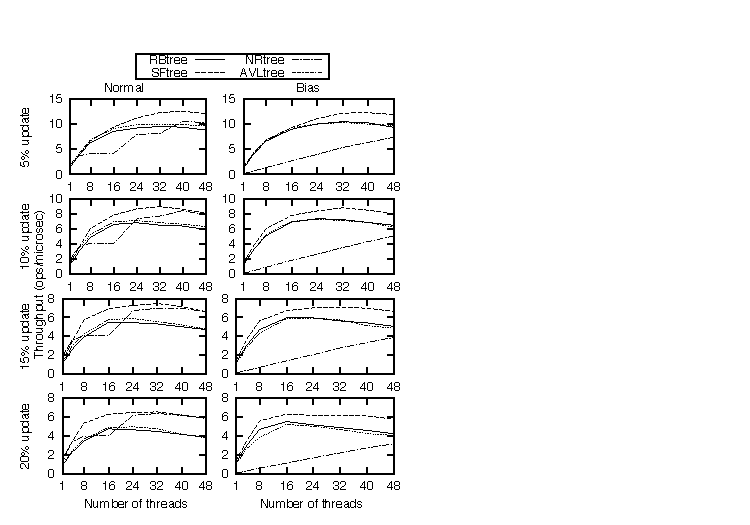
\includegraphics[scale=1.2,clip=true,viewport=9 0 192 228]{Tree/fig/microbench/microbench_avg_4096}
	\caption{Comparing the AVL tree (AVLtree), the red-black tree (RBtree), the no-restructuring tree (NRtree) against the speculation-friendly tree (SFtree) on an integer set micro-benchmark with from 5\% {\bf (top)} to 20\% updates {\bf (bottom)} under normal {\bf (left)} and biased {\bf (right)}  workloads\label{fig:microbench}}
	\end{center}
\end{figure}

\subsection{Biased workloads and the effect of restructuring}\label{ssec:microbench}

In this section, we evaluate the performance of our speculation-friendly tree on an integer set micro-benchmark providing $\act{remove}$, $\act{insert}$, and $\act{contains}$ operations, similarly to the benchmarks used to evaluate state-of-the-art TM algorithms~\cite{FFR08,FGG09,DSS10}.
We implemented two set libraries that we added to the synchrobench distribution:
(1) our non-optimized speculation-friendly tree and (2) a baseline tree that is similar but never rebalances the structure whatever modifications occur.
% our non-optimized speculation-friendly tree and a baseline tree that is similar but never rebalances the structure whatever modifications occur.
Figure~\ref{fig:microbench} depicts the performance obtained from four different binary search trees: the red-black tree (RBtree), our speculation-friendly tree without optimizations (SFtree), the no-restructuring tree (NRtree) and the AVL tree (AVLtree). 

% The performance is expressed as the number of operations executed per microsecond. The update ratio varies between 5\% and 20\%. As we obtained similar results with $2^{10}$, $2^{12}$ and $2^{14}$ elements, we only report the results obtained from an initialized set of $2^{12}$ elements.
% The biased workload consists of inserting (resp. deleting) random values skewed towards high (resp. low) numbers in the value range: the values always taken from a range of $2^{14}$ are skewed with a fixed probability by incrementing (resp. decrementing) with an integer uniformly taken within $[0..9]$.
The performance is expressed as the number of operations executed per microsecond. The update ratio varies between 5\% and 20\%.
As we obtained similar results with $2^{10}$, $2^{12}$ and $2^{14}$ elements, we only report the results obtained from an initialized set of $2^{12}$ elements.
We tested the algorithms using two workloads:
(1) The normal workload in which elements are inserted (resp. deleted) by selecting values randomly with equal probability from the value range.
(2) The biased workload consists of inserting (resp. deleting) random values skewed towards high (resp. low) numbers in the value range:
the values always taken from a range of $2^{14}$ are skewed with a fixed probability by incrementing (resp. decrementing) with an integer uniformly taken within $[0..9]$.


On both the normal (uniformly distributed) and biased workloads, the speculation-friendly tree scales 
well up to 32/40 threads. The no-restructuring tree performance drops to a linear shape 
under the biased workload as expected: as it does not rebalance, the complexity increases with the length of the longest path from the root to a leaf that, in turn, increases with the 
number of performed updates.
In contrast, the speculation-friendly tree can only be unbalanced during a transient period of time which is too short to affect the performance 
even under biased workloads. 

The speculation-friendly tree improves both the red-black tree and the AVL tree performance by up to $1.5\times$ and $1.6\times$, respectively. 
The speculation-friendly tree is less prone to contention than AVL and red-black trees, which both share similar performance penalties due to contention.


\begin{figure}
	\begin{center}
	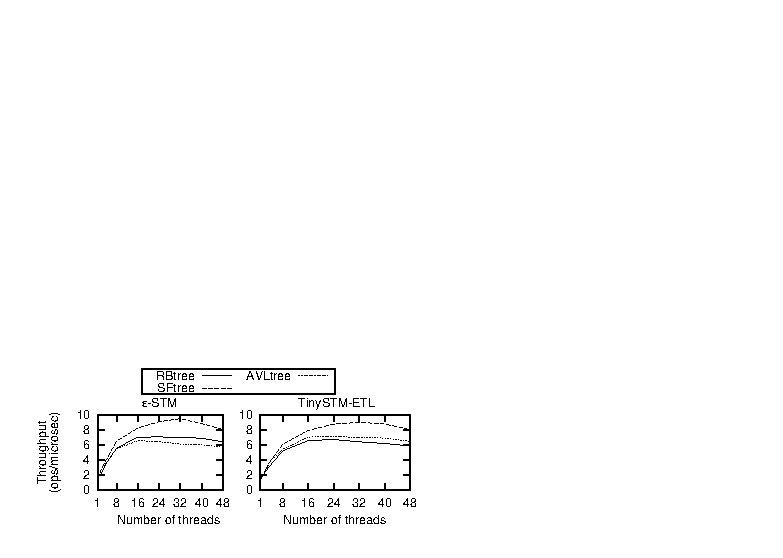
\includegraphics[scale=1.6,clip=true,viewport=0 0 200 83]{Tree/fig/microbench/microbench_avg_4096_u10_estm}
	\caption{The speculation-friendly library running with {\bf (left)} another TM library (${\mathcal E}$-STM) and with {\bf (right)} the previous TM library in a different configuration (TinySTM-ETL, i.e., with eager acquirement)\label{fig:estm}} 
	\end{center}
\end{figure}

\subsection{Portability to other TM algorithms}\label{ssec:othertms}

The speculation-friendly tree is an inherently efficient data structure that is portable to any TM systems.
It fulfills the TM interface standardized in~\cite{abi} and thus does not require the presence of explicit
escape mechanisms like early $\lit{release}$~\cite{HLMS03} or $\lit{snap}$~\cite{CH05} to avoid extra TM bookkeeping 
(our $\act{uread}$ optimization being optional).
Nor does it require high-level conflict detection, like open nesting~\cite{Mos06,NMA+07,ALS09} or transactional boosting~\cite{HK08}. Such improvements rely on 
explicit calls or user-defined abstract locks, and are not supported by existing TM compilers~\cite{abi} which limits their portability.
%
To make sure that the obtained results are not biased by the underlying TM algorithm,
we evaluated the trees on top of ${\mathcal E}$-STM~\cite{FGG09}, another TM library (on a $2^{16}$ sized tree where ${\mathcal E}$-STM proved efficient),
and on top of a different TM design from the one used so far: with eager acquirement.

The obtained results, depicted in Figure~\ref{fig:estm} look similar to the ones obtained with TinySTM-CTL
(Figure~\ref{fig:microbench}) in that the speculation-friendly tree executes faster than other trees for all TM settings.
This suggests that the improvement of speculation-friendly tree 
is potentially independent from the TM system used.
A more detailed comparison of the improvement obtained
using elastic transactions on red-black trees against the improvement of replacing the red-black tree by the speculation-friendly tree
is depicted in Figure~\ref{fig:move1}. It shows that the elastic improvements (15\% on average) is lower than the 
speculation-friendly tree one (22\% on average, be it optimized or not). 

\subsection{Reusability for specific application needs}

We illustrate the reusability of the speculation-friendly tree by composing $\act{remove}$ and $\act{insert}$ from the existing interface to obtain a new
atomic and deadlock-free $\act{move}$ operation.
Reusability is appealing to simplify concurrent programming by making it modular:
a programmer can reuse a library without having to understand its synchronization internals.
While reusability of sequential programs is straightforward, concurrent programs can generally be reused only 
if the programmer understands how each element is protected. For example, reusing a library can lead to deadlocks
if shared data are locked in a different order than what is recommended by the library. Additionally, a lock-striping library
may not conflict with a concurrent program that locks locations independently even though they protect common locations, 
thus leading to inconsistencies.

\begin{figure}[t]
	\begin{center}
	\subfigure[Elastic transaction speedup vs. speculation-friendly tree speedup\label{fig:move1}]{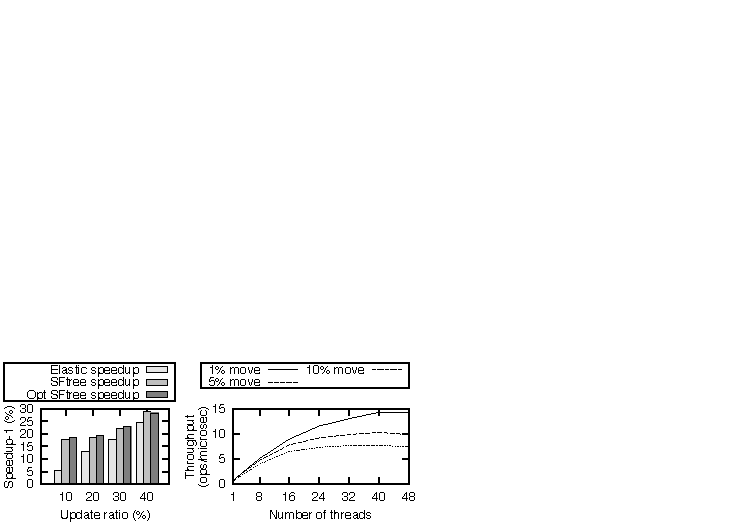
\includegraphics[scale=1.1,clip=true,viewport=0 0 84 78]{Tree/fig/microbench/microbench_65536_elastic_move}}\hspace{1em}
	\subfigure[Performance when reusing the speculation-friendly tree\label{fig:move2}]{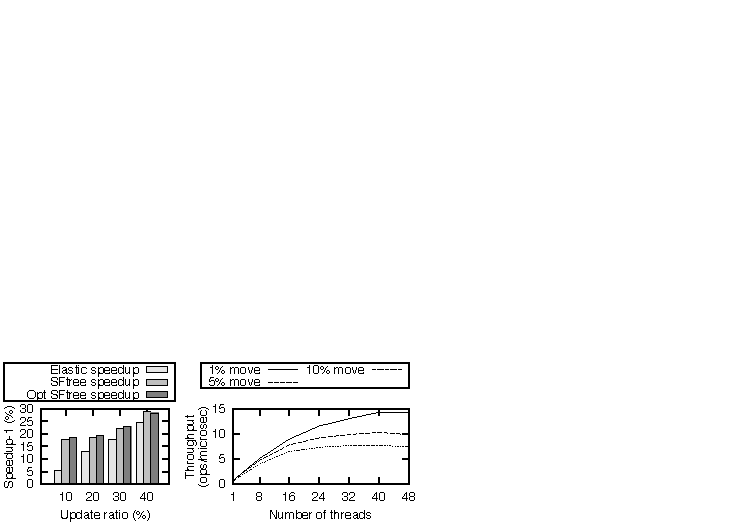
\includegraphics[scale=1.1,clip=true,viewport=89 0 200 78]{Tree/fig/microbench/microbench_65536_elastic_move}}
	\caption{Elastic transaction comparison and reusability}
	\end{center}
\end{figure}

Figure~\ref{fig:move2} indicates the performance on workloads comprising $90\%$ of read-only operations (including $\act{contains}$ and failed updates) and $10\%$ $\act{move}$/$\act{insert}$/$\act{delete}$ effective update operations (among which from $1\%$ to $10\%$ are $\act{move}$ operations).
The performance decreases as more 
$\act{move}$ operations execute, because a $\act{move}$ protects more elements in the data structure 
than a simple $\act{insert}$ or $\act{delete}$ operation and during a longer period of time.  

\subsection{The vacation travel reservation application}

We experiment our optimized library tree with a travel reservation application 
from the STAMP suite~\cite{CCKO08}, called vacation.
This application is suitable for evaluating concurrent binary search tree as it 
represents a database with four tables implemented as tree-based directories (cars, rooms, 
flights, and customers) accessed concurrently by client transactions. 

Figure~\ref{fig:vacation-threads} depicts the execution time of the STAMP vacation application
building on the Oracle red-black tree library (by default), 
our optimized speculation-friendly tree, 
and the baseline no-restructuring tree. 
We added the speedup obtained with each of these tree libraries over the performance of bare sequential code of vacation without synchronization.
(A concurrent tree library outperforms the sequential tree when its speedup exceeds 1.)
The chosen workloads are the two default configurations (``low contention'' and ``high contention'') 
taken from the STAMP release, with the default number of transactions, $8\times$ more transactions than by default and $16\times$ 
more, to increase the duration and the contention of the benchmark without using more threads than cores.

\begin{figure}[t]	
	\begin{center}
	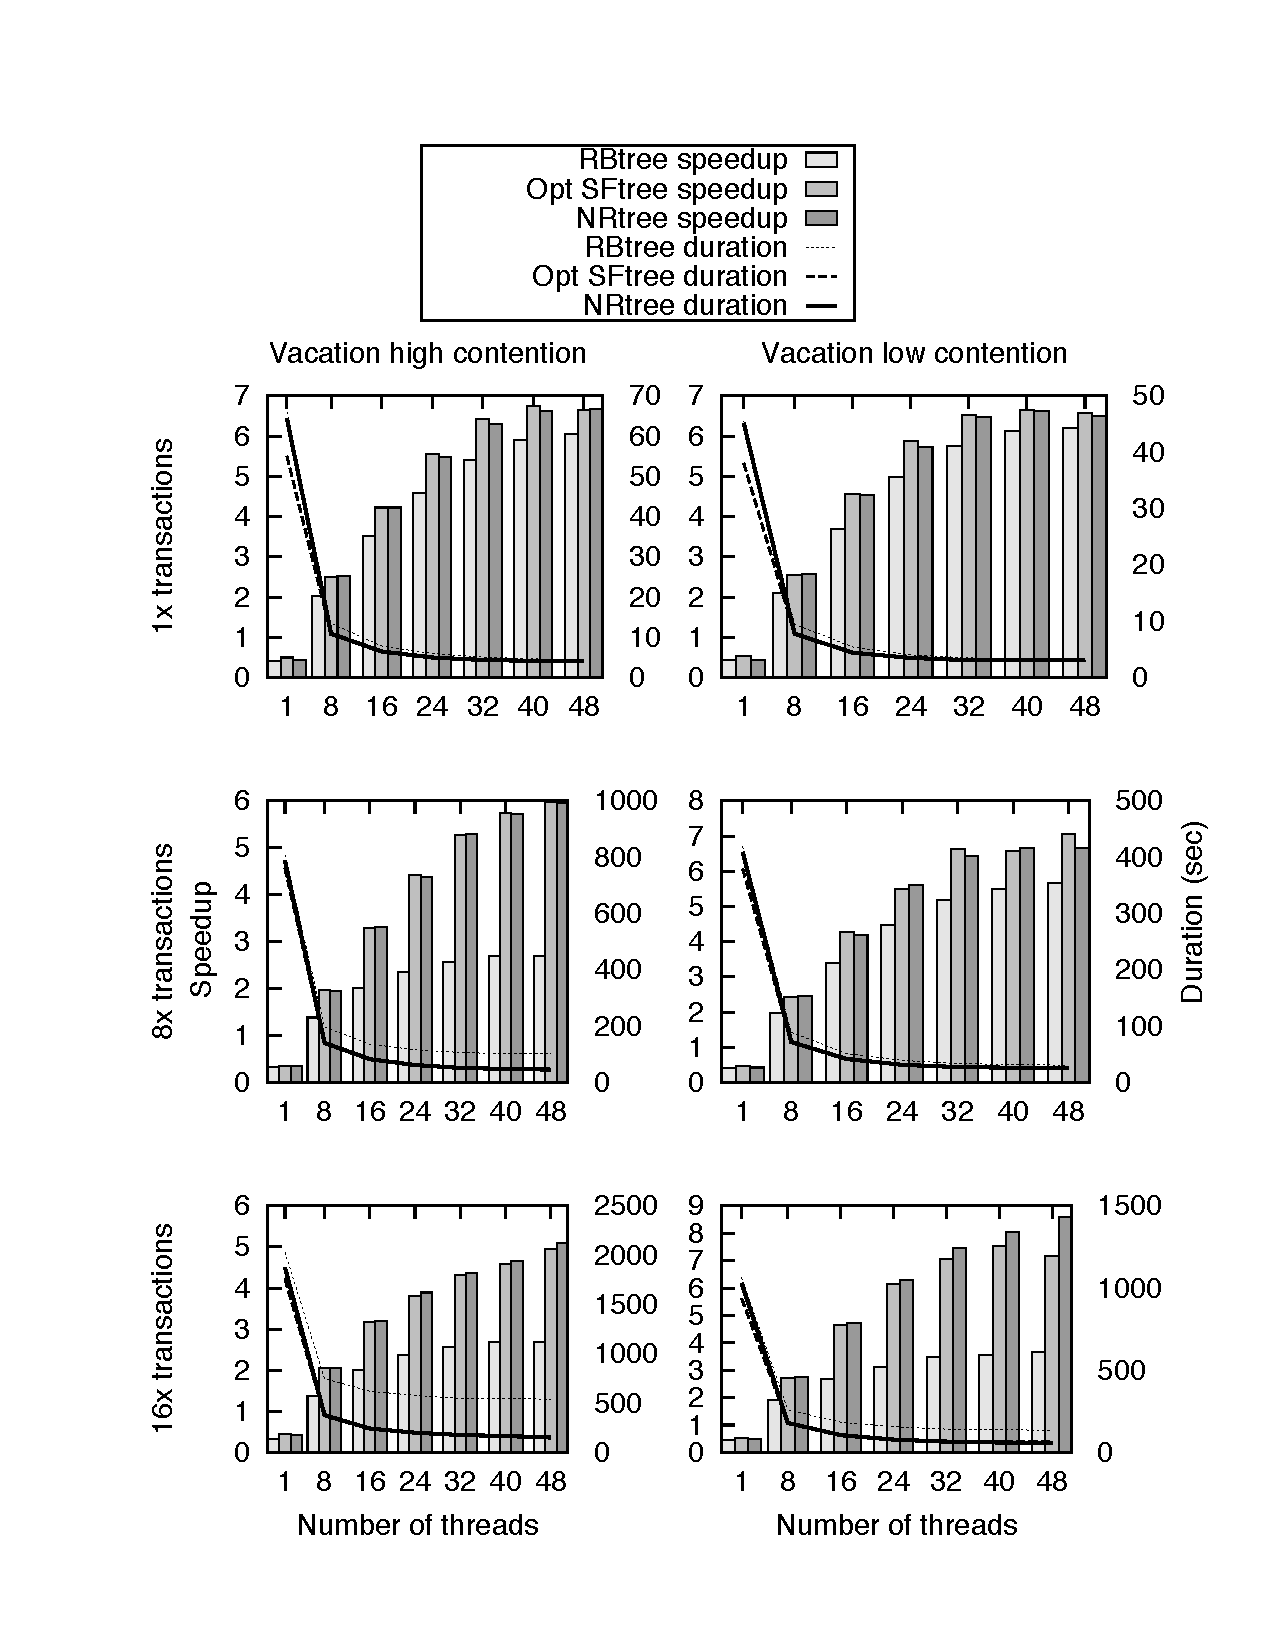
\includegraphics[scale=0.4,clip=true,viewport=49 5 580 750]{Tree/fig/vacation/vacation_avg2}
	\caption{The speedup (over single-threaded sequential) and the corresponding duration of the vacation application built upon the red-black tree (RBtree), the optimized speculation-friendly tree (Opt SFtree) and the no-restructuring tree (NRtree) on  {\bf (left)} high contention and  {\bf (right)} low contention workloads, and with  {\bf (top)} the default number of transaction,  {\bf (middle)} $8\times$ more transactions and {\bf (bottom)} $16\times$ more transactions\label{fig:vacation-threads}}	
	\end{center}
\end{figure}


Vacation executes always faster on top of our speculation-friendly tree than on top of its built-in Oracle red-black tree. 
For example, the speculation-friendly tree improves performance by up to $1.3\times$ with the default 
number of transactions and to $3.5\times$ with $16\times$ more transactions.
%
The reason of this is twofold: 
(i)~In contrast with the speculation-friendly tree, if an operation on the red-black tree traverses a location that is being 
deleted, then this operation and the deletion conflict. (ii)~Even though the Oracle red-black tree tolerates that the longest 
path from the root to a leaf can be twice as long as the shortest one, it triggers the rotation immediately after this threshold
is reached. By contrast, our speculation-friendly tree keeps checking the unbalance to potentially rotate in the background.
In particular, 
we observed on 8 threads in the high contention settings that the red-black tree vacation triggered around 
$130,000$ rotations whereas the speculation-friendly vacation triggered only $50,000$ rotations.

Finally, we observe that vacation presents similarly good performance on top of the no-restructuring tree library.
In rare cases, the speculation-friendly tree outperforms the no-restructuring tree probably because the no-restructuring tree
does not physically remove nodes from the tree,  thus leading to a larger tree than the abstraction.
Overall, their performance is comparable. With $16\times$ the default number of transactions,
the contention gets higher and rotations are more costly.

\section{Related Work}\label{sec:rw}

Aside from the optimistic synchronization context, various relaxed balanced trees have been proposed.
The idea of decoupling the update and the rebalancing was originally 
proposed by Guibas and Sedgewick~\cite{GS78} and was applied to AVL trees by Kessels~\cite{Kes83}, and 
Nurmi, Soisalon-Soininen and Wood~\cite{NSW87},
and to red-black trees by Nurmi and Soisalon-Soininen~\cite{NS98}.
Manber and Ladner propose a lock-based tree whose rebalancing is the task of separate maintenance threads running with a 
low priority~\cite{UR84}.  
Boug\'e et al.~\cite{IRISAppr} propose to lock a constant number of nodes within local rotations. 
The combination of local rotations executed by different threads self-stabilizes to a tree where no nodes are marked for removal.
The main objective of these techniques is still to keep the tree depth low enough for the lock-based operations to be efficient.
Such solutions do not apply to speculative operations due to aborts.
 
Ballard~\cite{Bal06} proposes a relaxed red-black tree insertion well-suited for transactions.
When an insertion unbalances the red-black tree it marks the inserted node rather than rebalancing the tree immediately. 
Another transaction encountering the marked node must rebalance the tree before restarting.
The relaxed insertion was shown generally more efficient than the original insertion 
when run with DSTM~\cite{HLMS03} on 4 cores. Even though the solution limits the waste of effort per aborting rotation, it increases the number of restarts per rotation.
By contrast, our local rotation does not require the rotating transaction to restart, hence benefiting both insertions and removals.

Bronson et al.~\cite{BCCO10} introduce an efficient object-oriented binary search tree. The algorithm uses underlying time-based TM principles to achieve good performance, 
however, its operations cannot be encapsulated within transactions. For example, a key optimization of this tree distinguishes
whether a modification at some node $i$ grows or shrinks the subtree rooted in $i$. A conflict involving a growth could be ignored as no descendant are removed
and a $\lit{search}$ preempted at node $i$ will safely resume in the resulting subtree.
Such an optimization is not possible using TMs that track conflicts between read/write accesses to the shared memory.
This implementation choice results in higher performance by avoiding the TM overhead, but limits reusability due to the lack of bookkeeping.
%
For example, a programmer willing to implement a $\lit{size}$ operation would need to explicitly $\lit{clone}$ the data structure to disable the growth optimization.
Therefore, the programmer of a concurrent application that builds upon this binary search tree library must be aware of the synchronization internals of this library 
(including the growth optimization) to reuse it.

Felber, Gramoli and Guerraoui~\cite{FGG09} specify the elastic transactional model that ignores false conflicts but guarantees reusability. 
In the companion technical report, 
the red-black tree library from Oracle Labs was shown executing efficiently on top of an implementation 
of the elastic transaction model, ${\mathcal E}$-STM. The implementation idea
consists of encapsulating the (i)~operations that locate a position in the red-black tree (like $\lit{insert}$, $\lit{contains}$, $\lit{delete}$) 
into an \emph{elastic} transaction to increase concurrency and (ii)~other operations, like $\lit{size}$, into a regular transaction.
This approach is orthogonal to ours as it aims at improving the performance of the underlying TM, independently from the data structure, by introducing relaxed transactions.
Hence, although elastic transactions can cut themselves upon conflict detection, the resulting ${\mathcal E}$-STM, still suffers from congestion and wasted work when applied to 
non-speculation-friendly data structures. The results presented in Section~\ref{ssec:othertms} confirm that the elastic speedup is even higher when the tree is speculation-friendly.

\section{Conclusion}\label{sec:conclusion}

Libraries are an important piece of concurrent programming
as they give programmers access to safe and efficient implementations
of popular abstractions such maps/dictionaries.
Given that through the transaction
abstraction STM provides a general purpose model for synchronization,
other abstractions such as the map/dictionary can be implemented from within transactions,
playing the role of synchronization toolboxes that a programmer can rely on to write 
a concurrent application easily.
Unfortunately due to the general speculative nature of synchronization provided by STM,
transaction-based data structures are becoming a bottleneck in multicore programming.
The work in that chapter shows that speculative executions require the design of new data structures.
The underlying challenge is to decrease the inherent contention by relaxing the invariants of the structure
while preserving the invariants of the abstraction.

In contrast with the traditional pessimistic synchronization, the optimistic synchronization allows us
to directly observe the impact of contention as part of the step complexity because conflicts potentially lead to subsequent speculative re-executions.
This chapter has illustrated, using a binary search tree, how one can exploit this information
to design a speculation-friendly data structure.
The next challenge is to
adapt this technique to a large body of data structures to derive a speculation-friendly library.
Providing such a library would encourage the use of STM for several reasons.
The most obvious being simply that a programmer would not have to create the data-structures himself,
preventing him from worrying about the correctness and efficiency of his code
thus helping ensure our goal of having STM as part of a complete concurrent ecosystem from Definition \ref{def:stm-def}.
Secondly, the programmer can compose several operations from the library within a transaction, creating
new operations specific to his needs, something that is normally not possible when using non-transactional data structures.
Thirdly, the library can be designed specifically for optimistic synchronization or take advantage of
non-standard TM operations such as the unit load.
Interesting this goes against our intended goal for the simplicity of the transaction interface
as desired by the Definition \ref{def:trans-def} of a transaction from the introduction.
Importantly though, the programmer using these libraries need not be aware of this non standard interface, thus allowing him to
gain performance advantages without knowing the underlying intricacies of the STM system, knowing only the
simple definition of a transaction.



\section*{Source Code}
The code of the speculation-friendly binary search tree is available at {\bf http://lpd.epfl.ch/gramoli/php/synchrobench.php}{http://lpd.epfl.ch/gramoli/php/synchrobench.php}.

% \section*{Acknowledgements}
% The research leading to these results has received funding from the European Union Seventh Framework Programme (FP7/2007-2013) under grant agreement number 238639, ITN project TransForm, and grant agreement number 248465, the S(o)OS project.
% 
% \bibliographystyle{plain}
% \bibliography{bib}
% 
% \end{document}
% \endinput

